\documentclass[10pt, a4paper]{article}

%%% SST LAB PROTOCOLL PREAMBLE
%%% 2019
%%%%%%%%%%%%%%%%%%%%%%%%%%%%%%%


%%% PACKAGES
%%%%%%%%%%%%%%%%%%%%%%%%%%%

\usepackage[ngerman]{babel}

\usepackage[utf8]{inputenc}
\usepackage{amsmath}
\usepackage{pgfplots}
\usepackage{tikz}
\usepackage[many]{tcolorbox}
\usepackage{graphicx}
\graphicspath{ {./graphics/} }
\usepackage{pdfpages}
\usepackage{dashrule}
\usepackage{float}
\usepackage{siunitx}
\usepackage{trfsigns}
\usepackage{booktabs}
\usepackage[european]{circuitikz}
\usepackage{tcolorbox}

%%% DOCUMENT GEOMETRY
%%%%%%%%%%%%%%%%%%%%%%%%%%%

\usepackage{geometry}
\geometry{
 a4paper,
 total={0.6180339887498948\paperwidth,0.6180339887498948\paperheight},
 top = 0.1458980337503154\paperheight,
 bottom = 0.1458980337503154\paperheight
 }
\setlength{\jot}{0.013155617496424828\paperheight}
\linespread{1.1458980337503154}

\setlength{\parskip}{0.013155617496424828\paperheight} % paragraph spacing


%%% COLORS
%%%%%%%%%%%%%%%%%%%%%%%%%%%

\definecolor{red1}{HTML}{f38181}
\definecolor{yellow1}{HTML}{fce38a}
\definecolor{green1}{HTML}{95e1d3}
\definecolor{blue1}{HTML}{66bfbf}
\definecolor{hsblue}{HTML}{00b1db}
\definecolor{hsgrey}{HTML}{afafaf}

%%% CONSTANTS
%%%%%%%%%%%%%%%%%%%%%%%%%%%
\newlength{\smallvert}
\setlength{\smallvert}{0.0131556\paperheight}


%%% COMMANDS
%%%%%%%%%%%%%%%%%%%%%%%%%%%

% differential d
\newcommand*\dif{\mathop{}\!\mathrm{d}}

% horizontal line
\newcommand{\holine}[1]{
  	\begin{center}
	  	\noindent{\color{hsgrey}\hdashrule[0ex]{#1}{1pt}{3mm}}\\%[0.0131556\paperheight]
  	\end{center}
}

% mini section
\newcommand{\minisec}[1]{ \noindent\underline{\textit {#1} } \\}

% quick function plot
\newcommand{\plotfun}[3]{
  \vspace{0.021286\paperheight}
  \begin{center}
    \begin{tikzpicture}
      \begin{axis}[
        axis x line=center,
        axis y line=center,
        ]
        \addplot[draw=red1][domain=#2:#3]{#1};
      \end{axis}
    \end{tikzpicture}
  \end{center}
}

% box for notes
\newcommand{\notebox}[1]{

\tcbset{colback=white,colframe=green1!100!black,title=Note!,width=0.618\paperwidth,arc=0pt}

 \begin{center}
  \begin{tcolorbox}[]
   #1 
  \end{tcolorbox}
 
 \end{center} 
 
}

% box for equation
\newcommand{\eqbox}[2]{
	
	\tcbset{colback=white,colframe=green1!100!black,title=,width=#2,arc=0pt}
	
	\begin{center}
		\begin{tcolorbox}[ams align*]
				#1
		\end{tcolorbox}
		
	\end{center} 
	
}
% END OF PREAMBLE

\addbibresource{sources.bib}

\begin{document}


\includepdf{./titlepage/titlepage.pdf}

\section*{Homework Tasks}
\begin{taskspec}

HW5)\\

due May 25th 23:59 LT\\

1)\\
- familiarize with antennas and antenna types (textbooks, wiki etc.)\\

2)\\
categorize and briefly summarize antenna types and their properties (gain, beam width, band width, impedance, characteristic sizes)\\

- single antennas: (nearly) omni-directional, directional (yagi, patch, parabolic dish)\\

- antenna groups (co-linear, antenna arrays)\\

include examples of corresponding radiation pattern\\
\end{taskspec}

\pagebreak

\section{Introduction}
final reporto


\section{Square 5x5 Array}

The following figures show the array factor patterns for a 5x5 planar antenna array with different spacings ($d$) and steering angles (either vertical or $\theta_{d}=60\,\si{\degree}$), calculated with python. The array geometry can be seen in figure \ref{fig:phase1}.\\

One can see grating lobes appear on the edges of some radiation patterns due to the finite antenna distances involved. As the distance between the antennas goes down, the angular distance towards the grating lobes increases, i.e. angular ambiguities appear ``later'' and the beam can be safely steered to greater angles. However, this also results in a greater beamwidth which might not be desired.\\

\begin{figure}[H]
  \begin{minipage}[t]{0.45\textwidth}
    \centering
    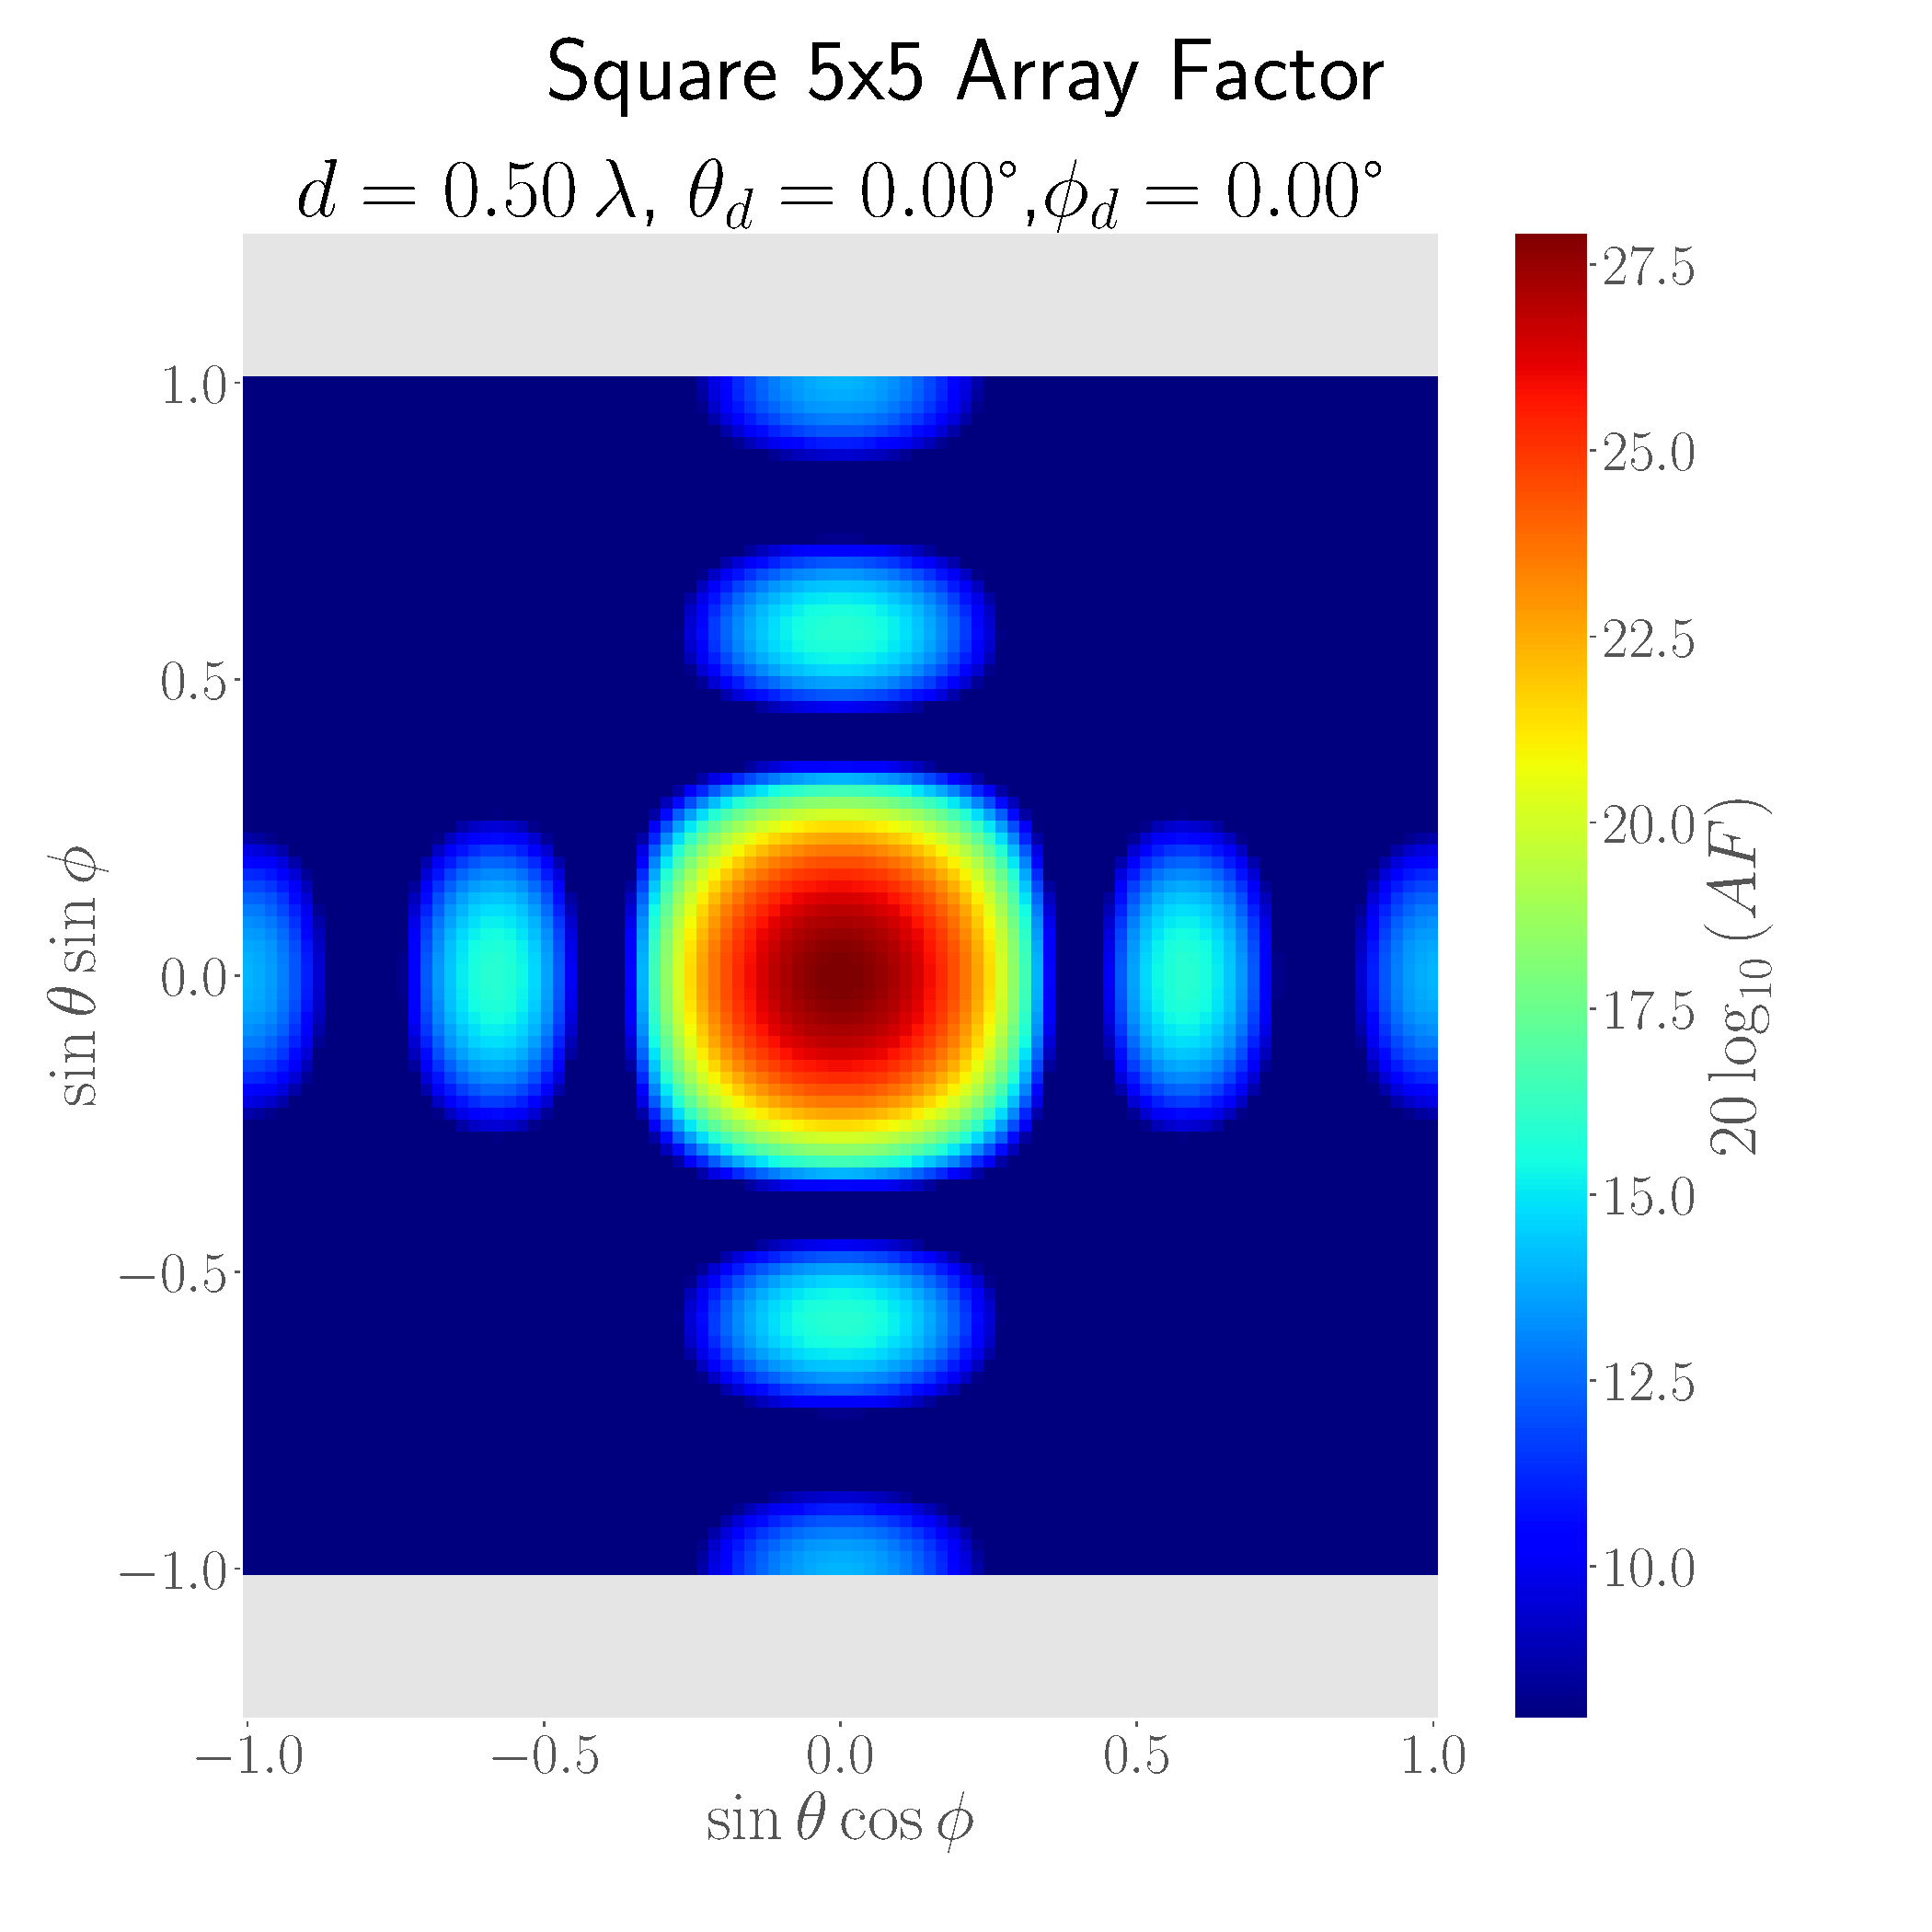
\includegraphics[width=\textwidth]{graphics/task_1/square-0.50-lambda-0.00-theta-0.00-phi-radpat.pdf}
    \caption{Square 5x5 vertically steered radiation pattern for $0.5\lambda$ spacing.}\label{fig:rad-square-0.5-0}
  \end{minipage}\hfill
  \begin{minipage}[t]{0.45\textwidth}
    \centering
    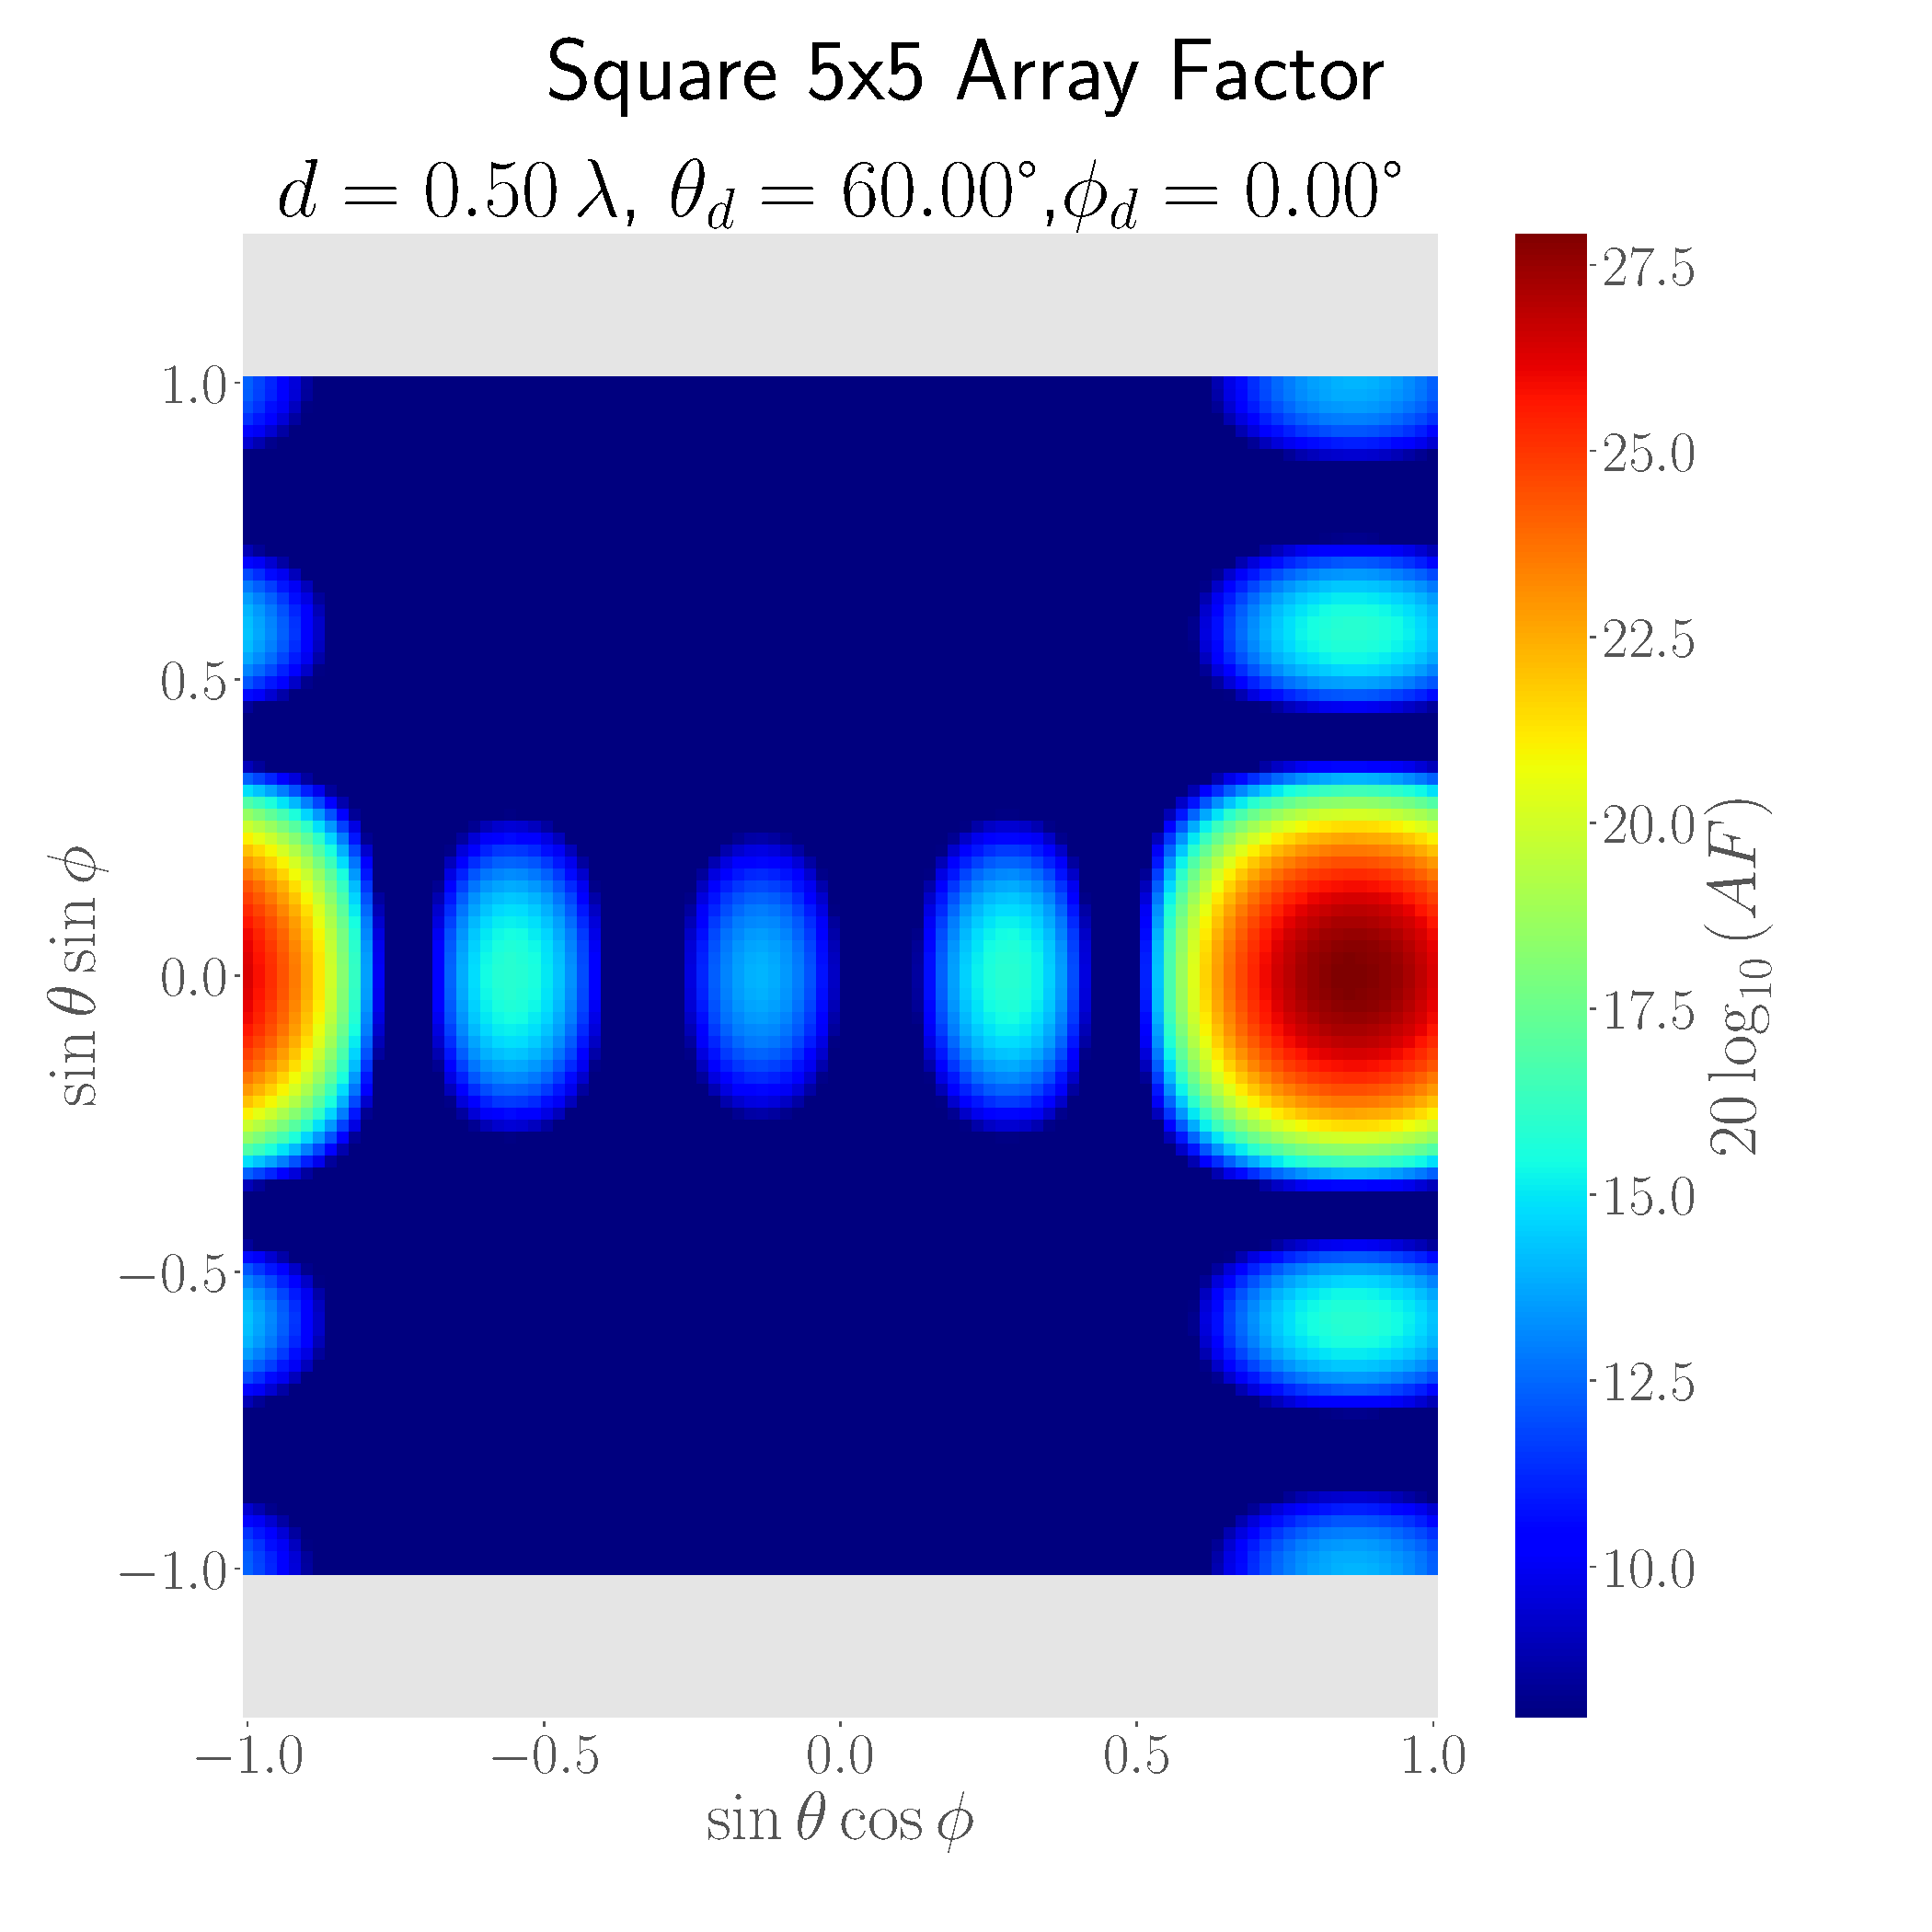
\includegraphics[width=\textwidth]{graphics/task_1/square-0.50-lambda-60.00-theta-0.00-phi-radpat.pdf}
    \caption{Square 5x5 off-vertically steered radiation pattern for $0.5\lambda$ spacing.}\label{fig:rad-square-0.5-60}
   \end{minipage}
\end{figure}

\begin{figure}[H]
  \begin{minipage}[t]{0.45\textwidth}
    \centering
    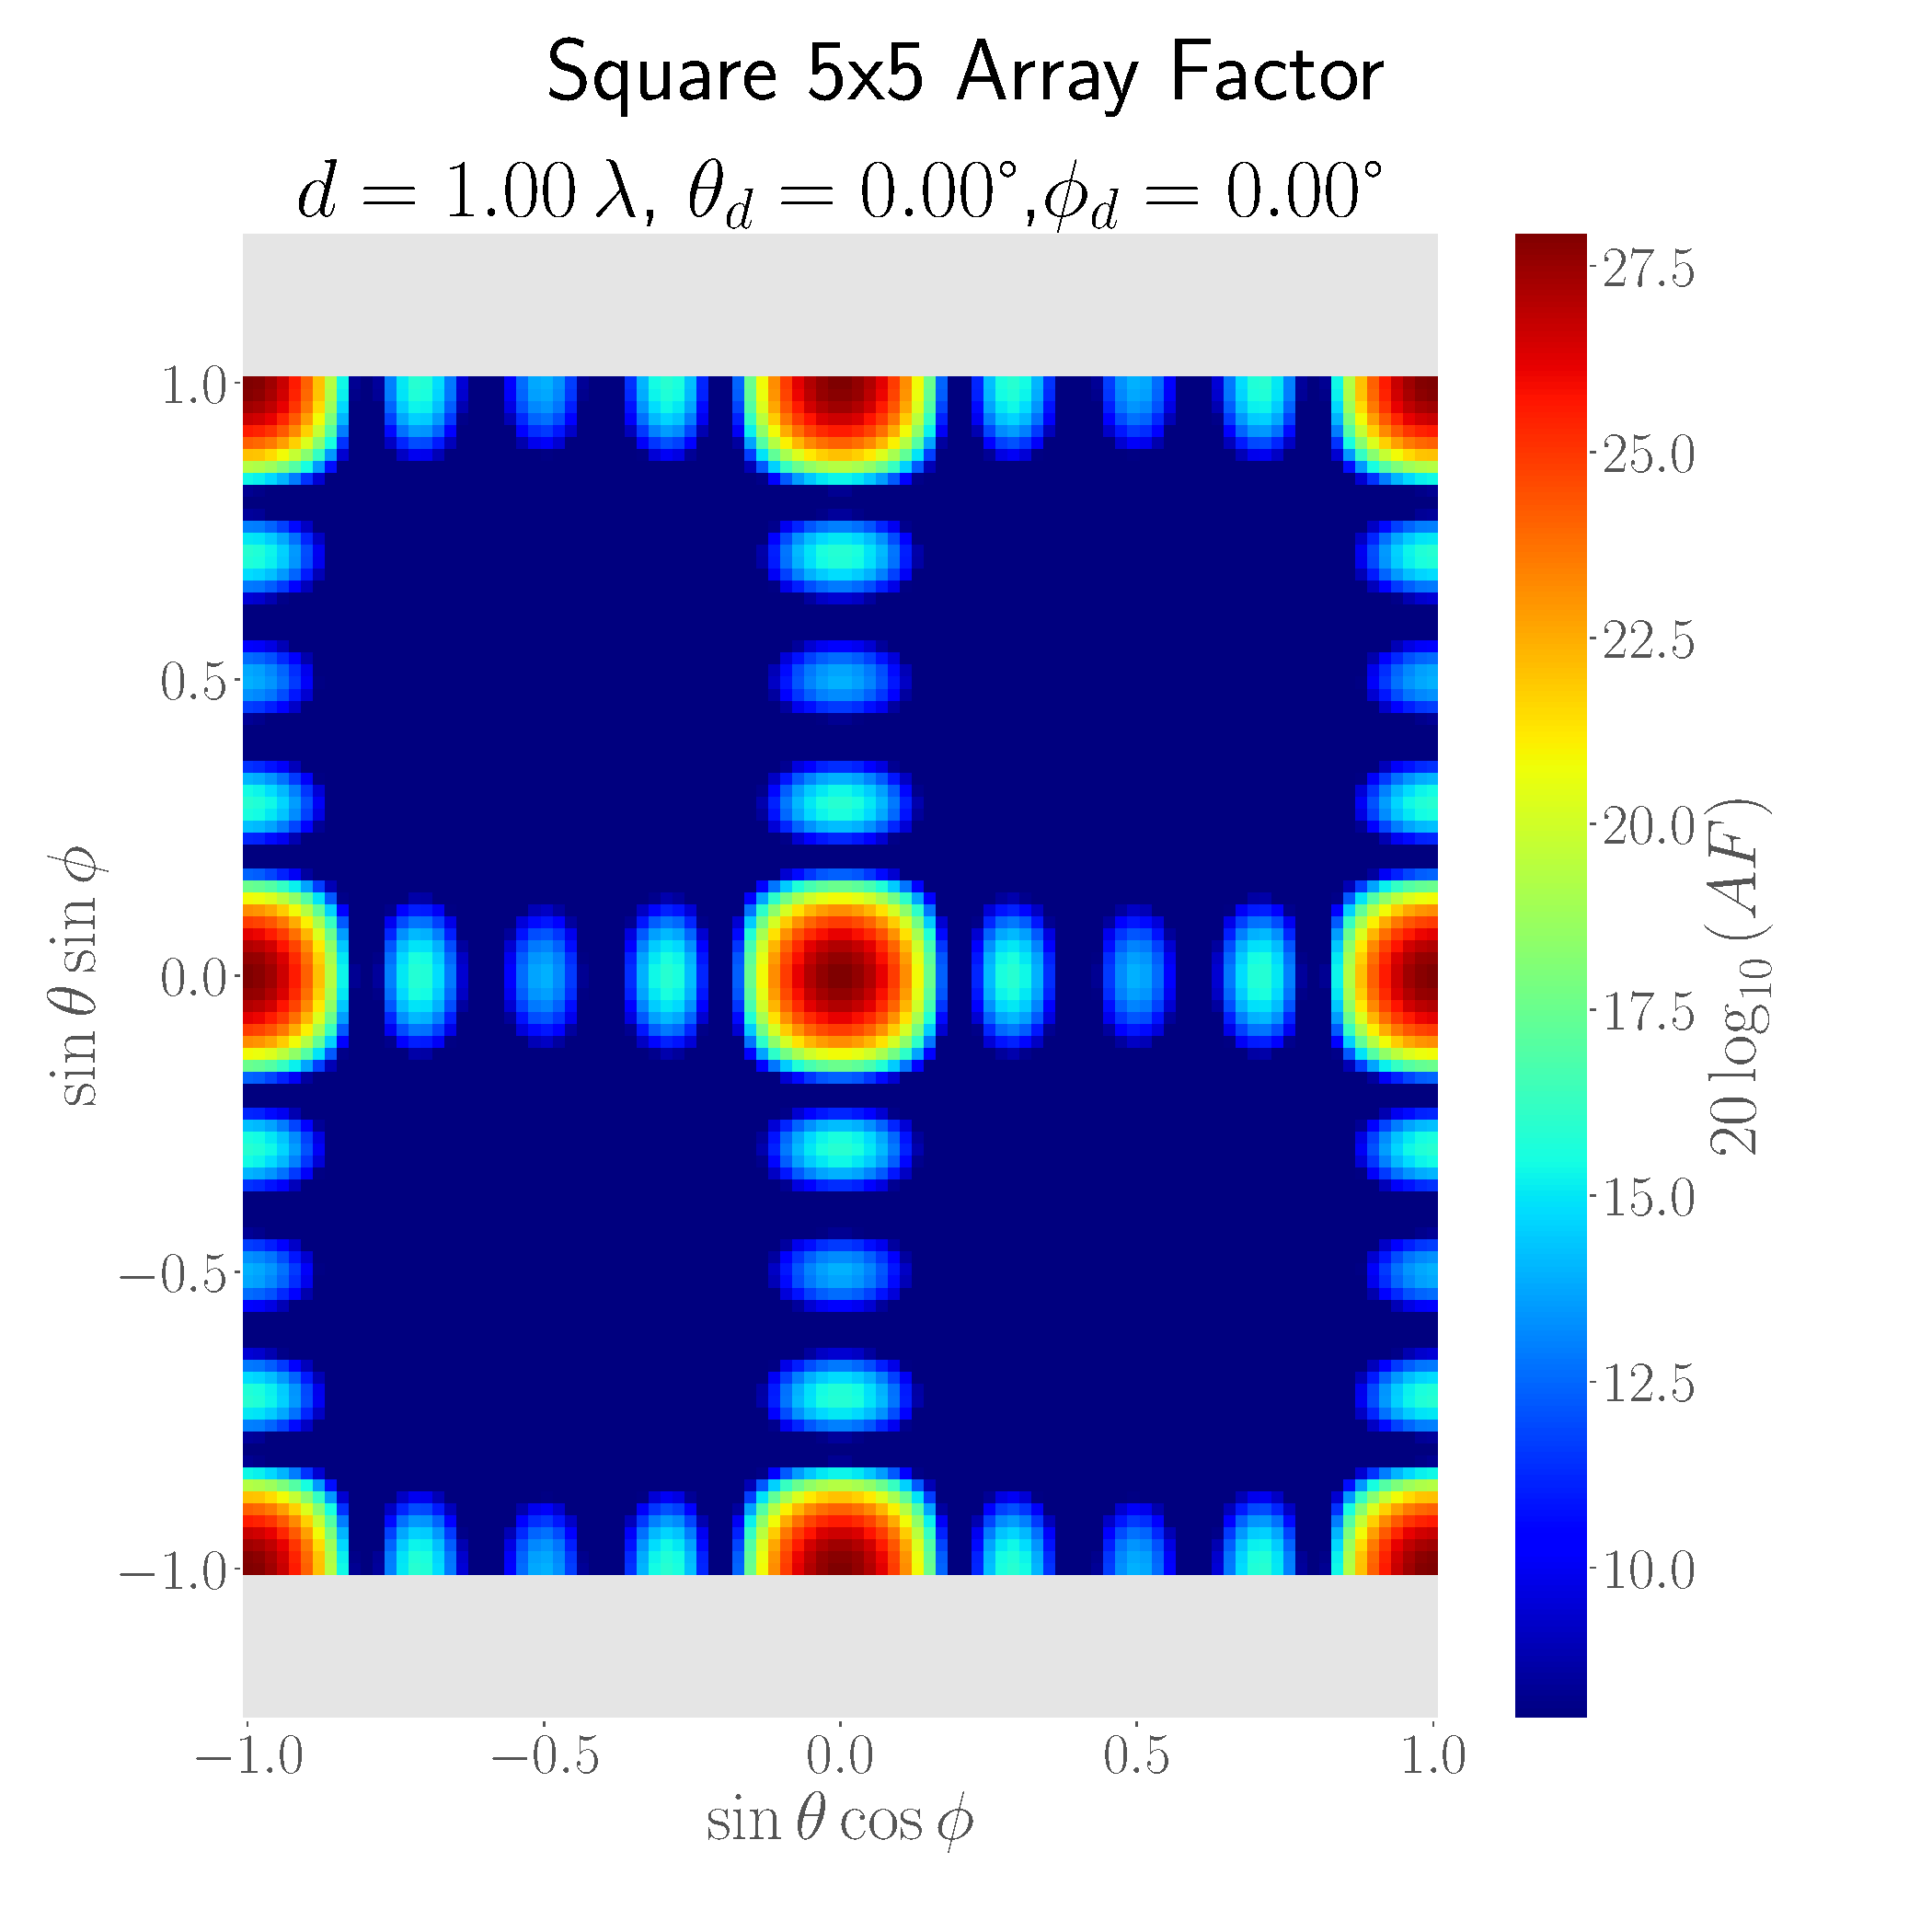
\includegraphics[width=\textwidth]{graphics/task_1/square-1.00-lambda-0.00-theta-0.00-phi-radpat.pdf}
    \caption{Square 5x5 vertically steered radiation pattern for $1.0\lambda$ spacing.}\label{fig:rad-square-1.0-0}
  \end{minipage}\hfill
  \begin{minipage}[t]{0.45\textwidth}
    \centering
    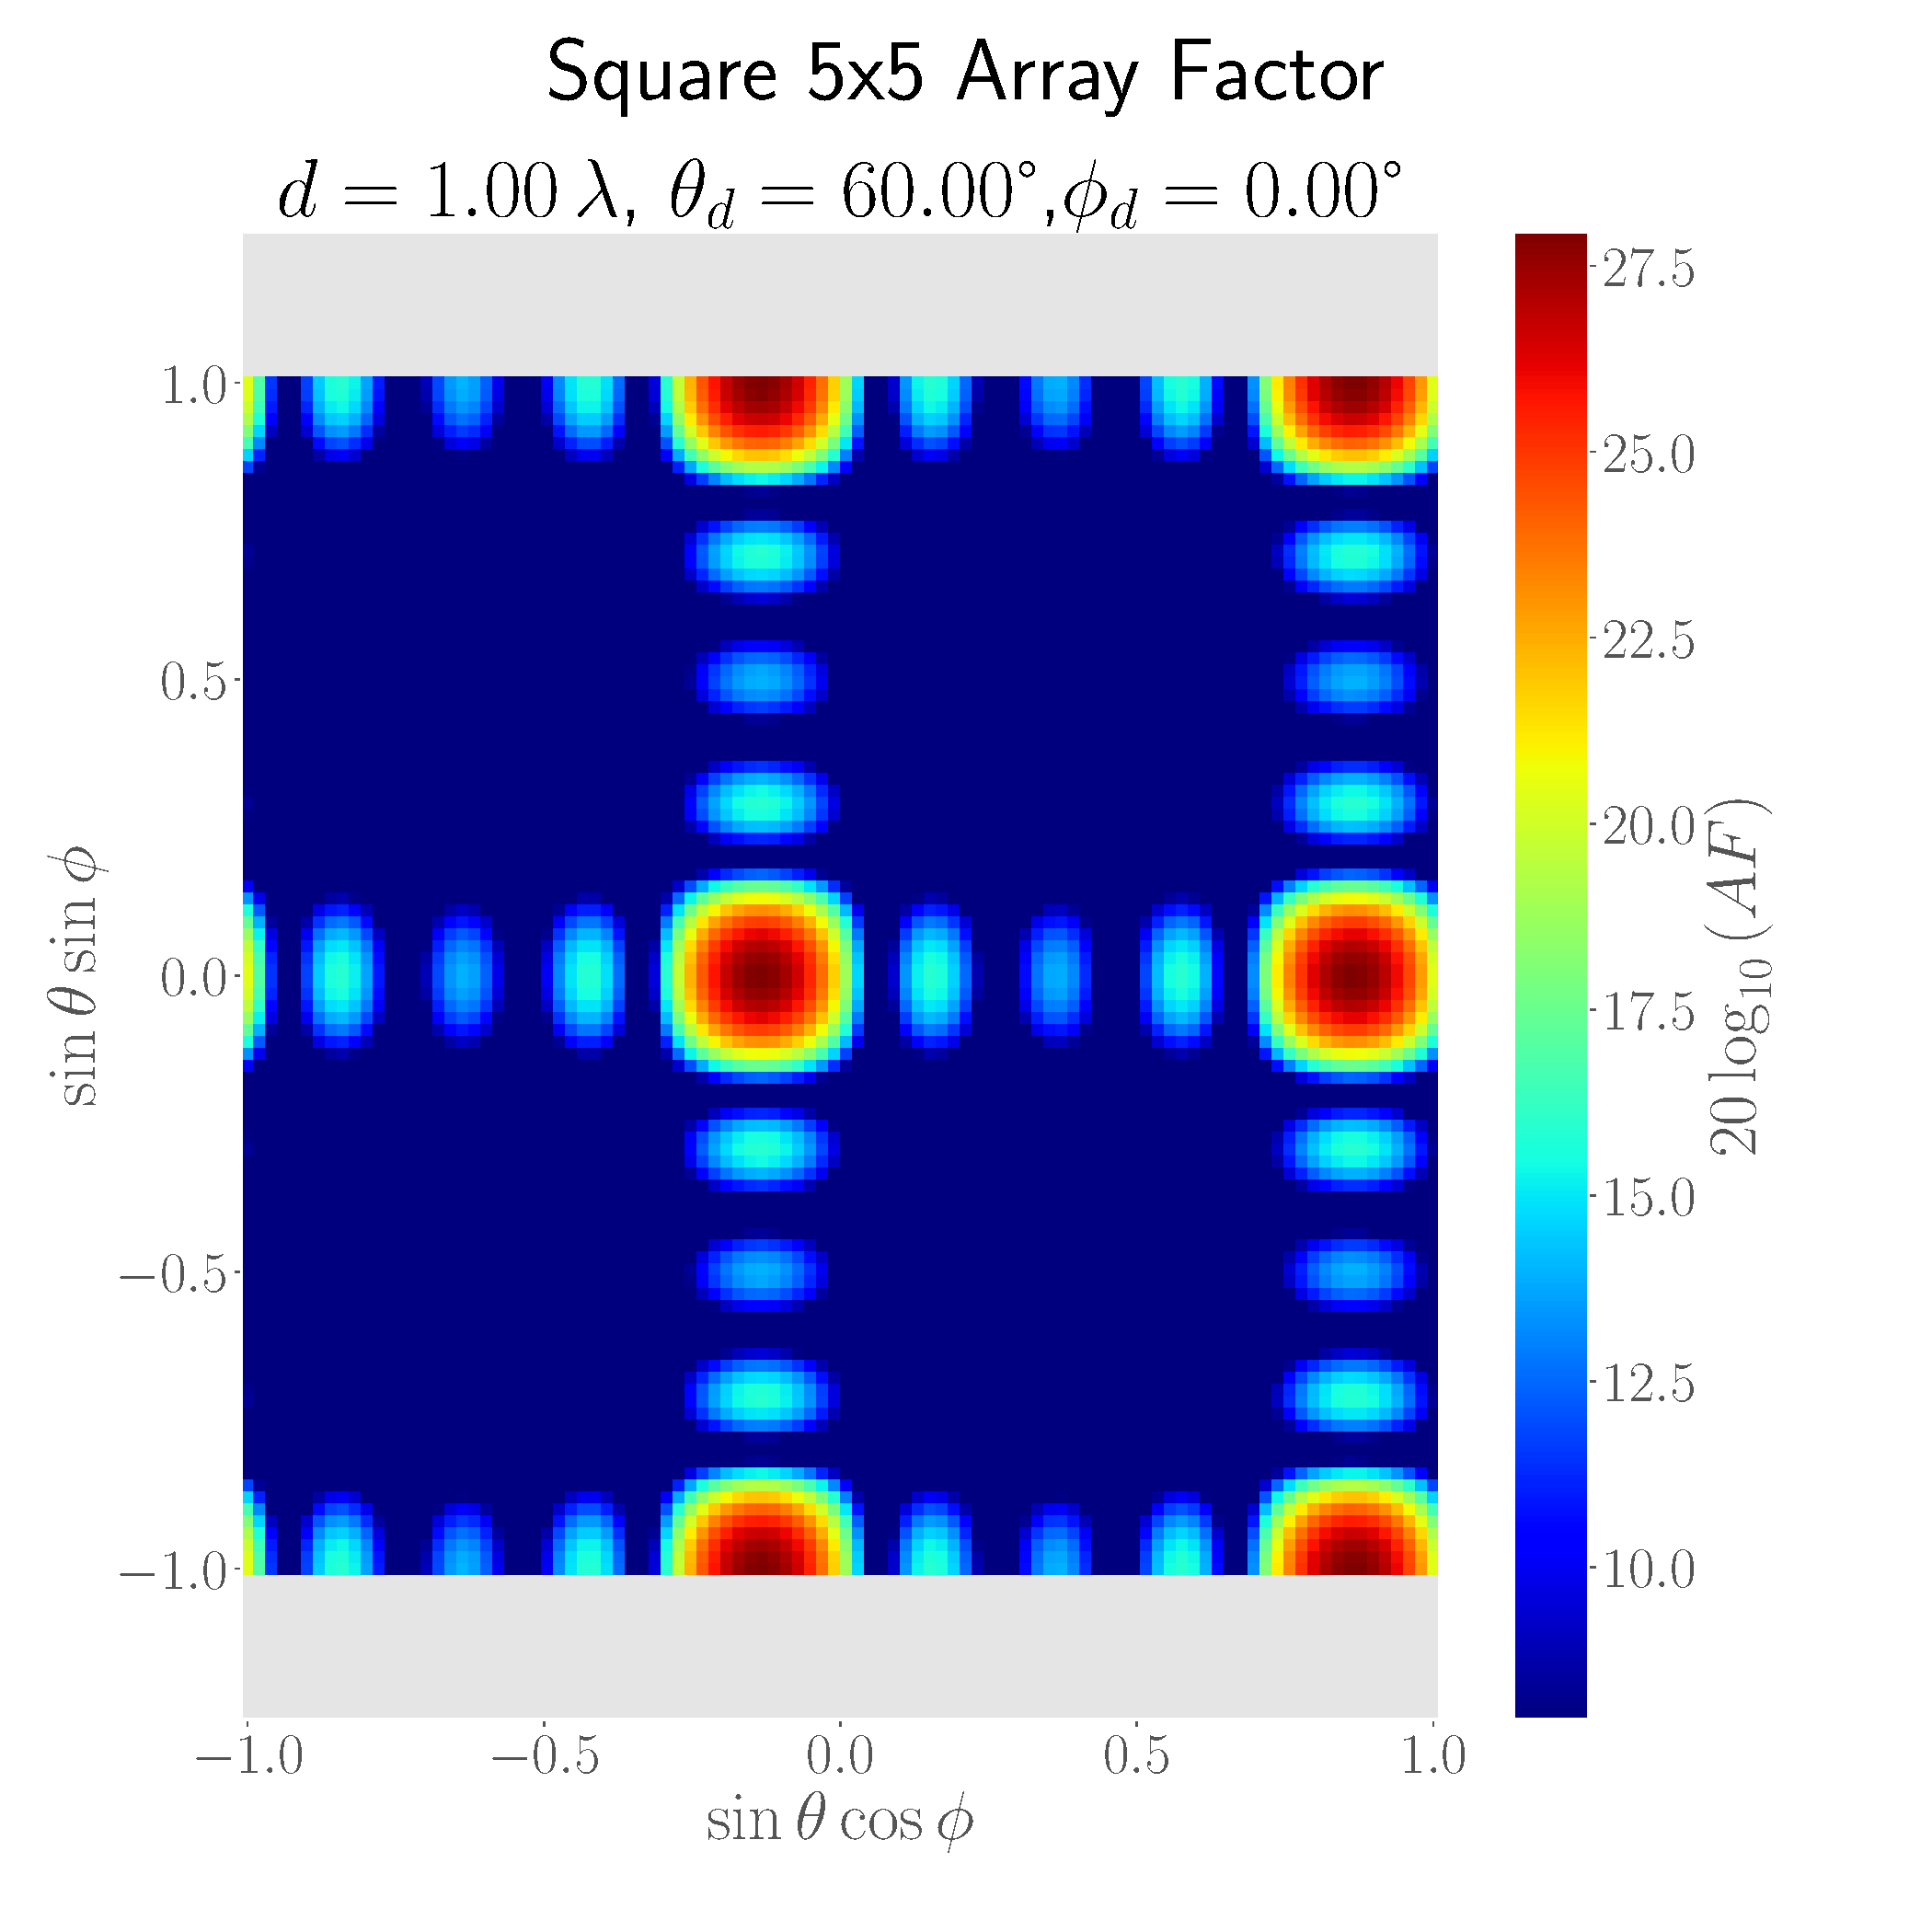
\includegraphics[width=\textwidth]{graphics/task_1/square-1.00-lambda-60.00-theta-0.00-phi-radpat.pdf}
    \caption{Square 5x5 off-vertically steered radiation pattern for $1.0\lambda$ spacing.}\label{fig:rad-square-1.0-60}
   \end{minipage}
\end{figure}

\begin{figure}[H]
  \begin{minipage}[t]{0.45\textwidth}
    \centering
    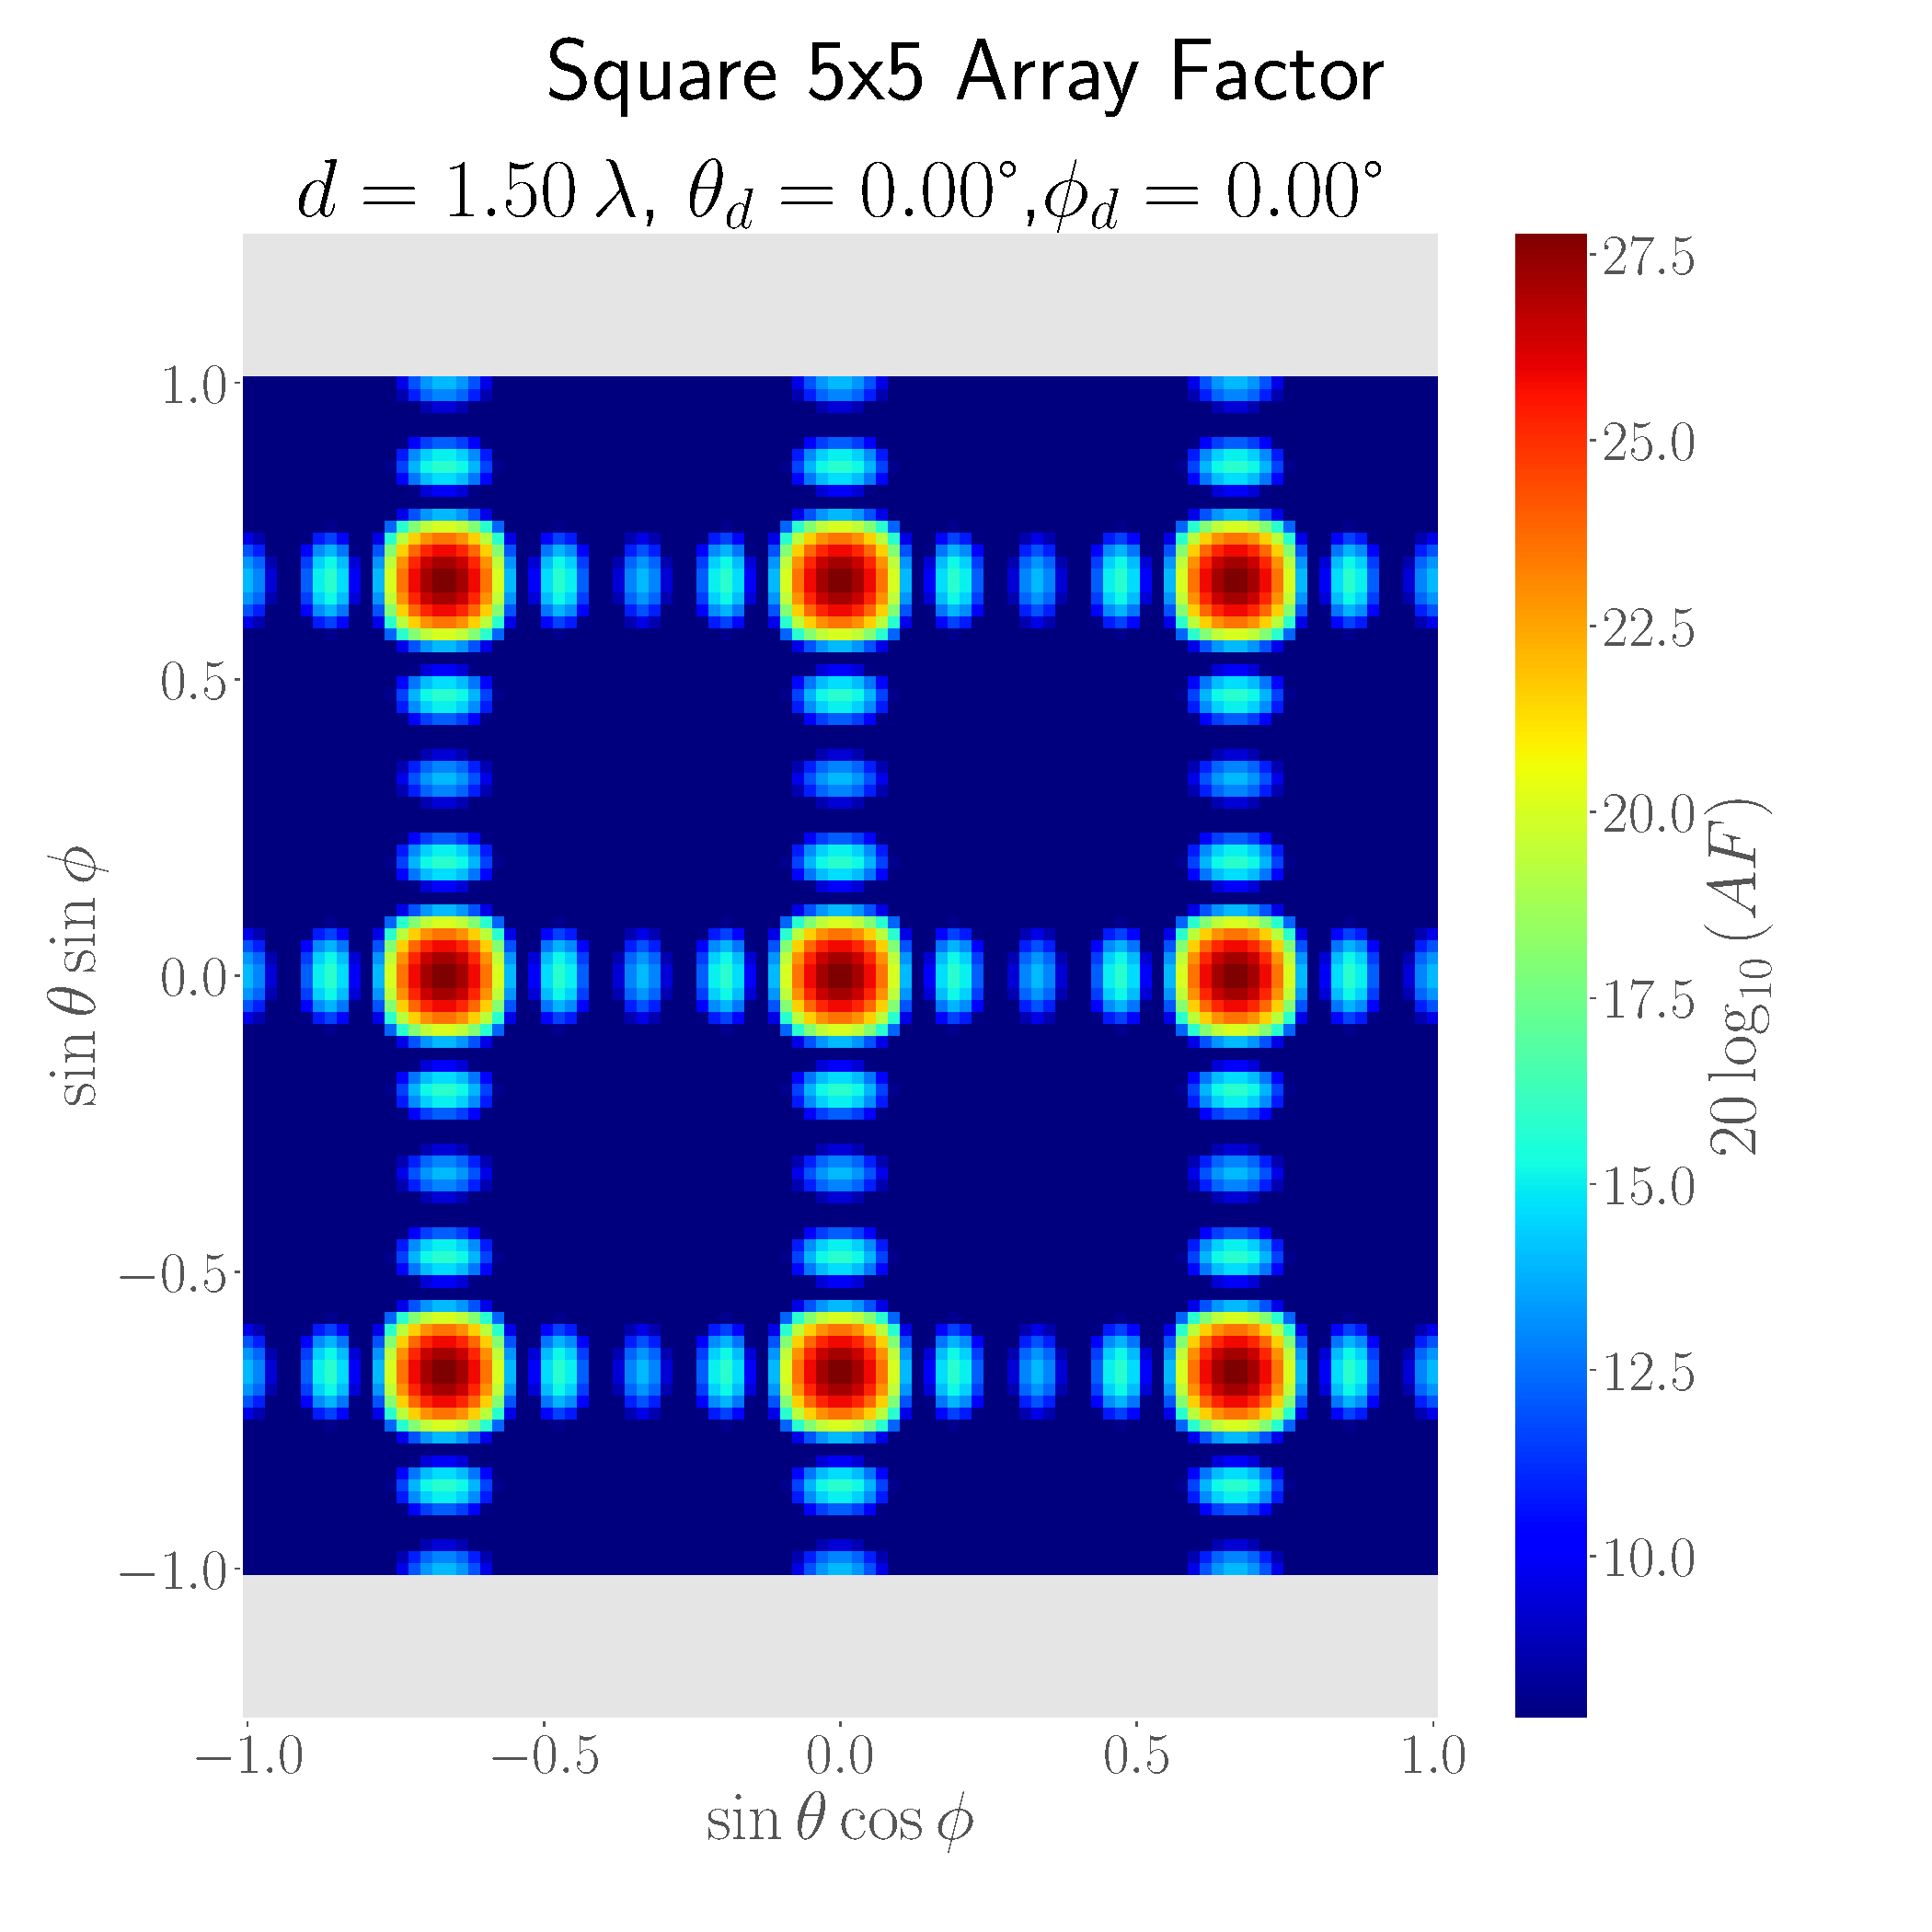
\includegraphics[width=\textwidth]{graphics/task_1/square-1.50-lambda-0.00-theta-0.00-phi-radpat.pdf}
    \caption{Square 5x5 vertically steered radiation pattern for $1.5\lambda$ spacing.}\label{fig:rad-square-1.5-0}
  \end{minipage}\hfill
  \begin{minipage}[t]{0.45\textwidth}
    \centering
    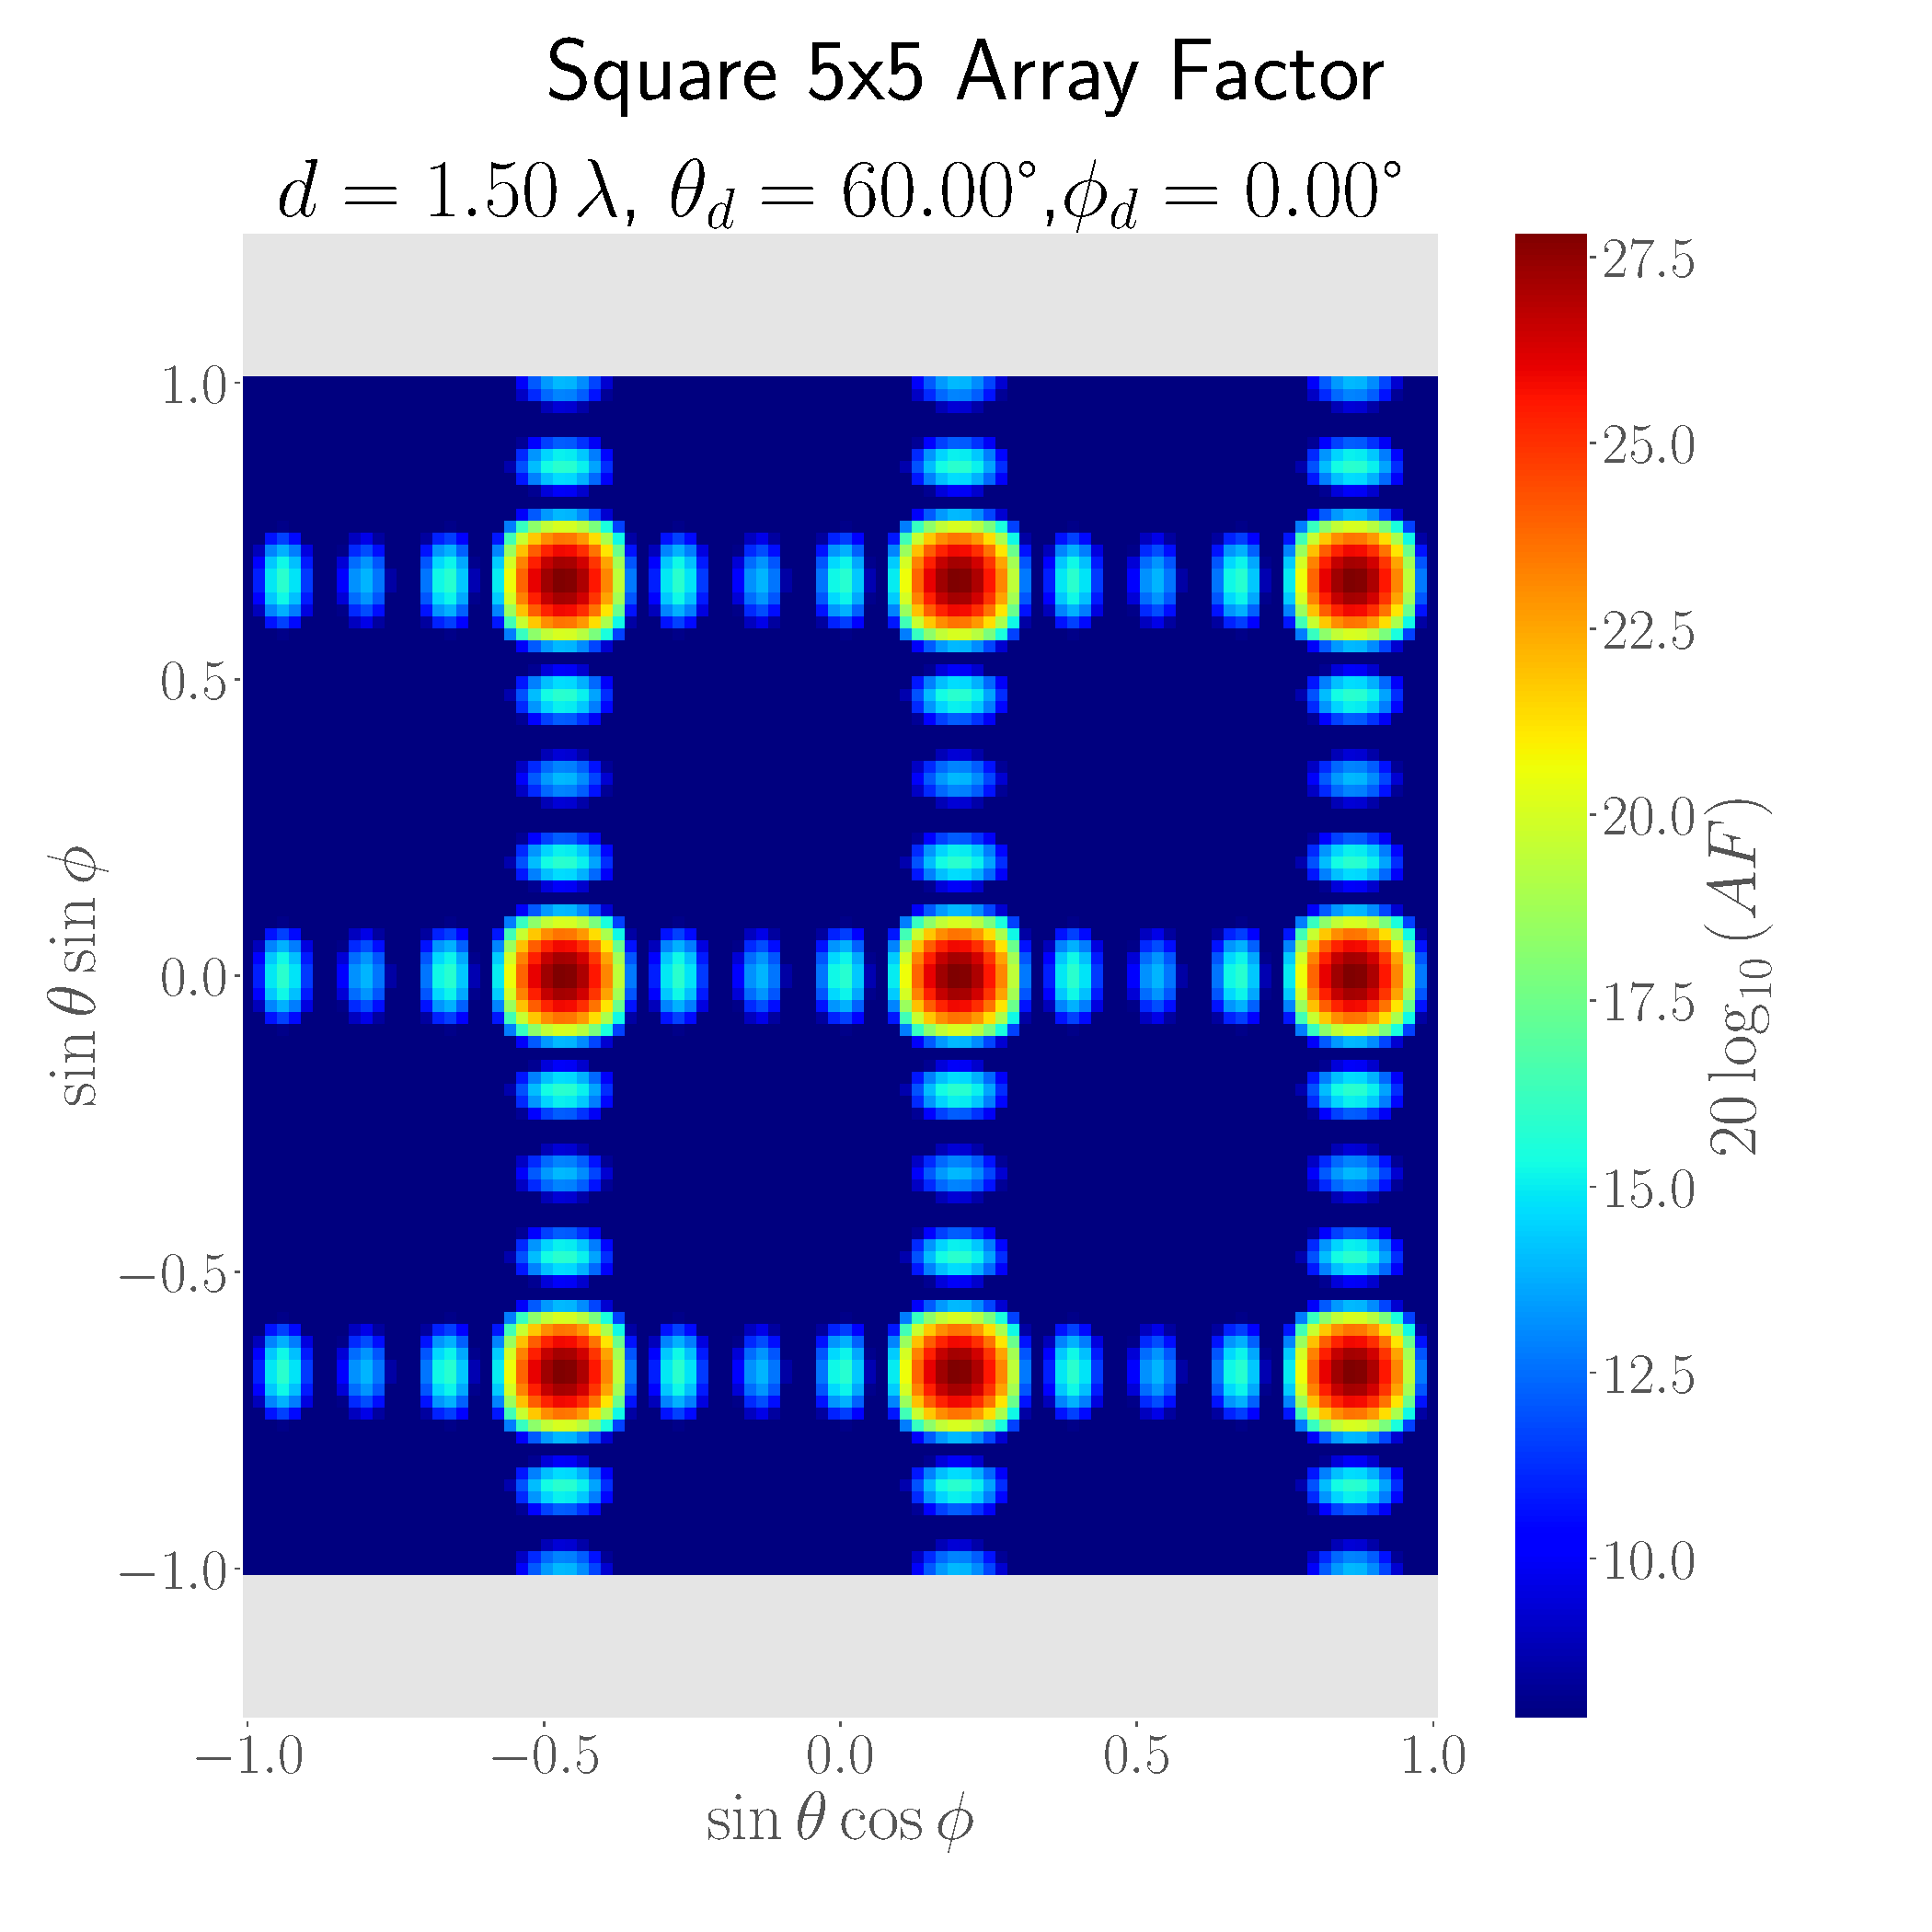
\includegraphics[width=\textwidth]{graphics/task_1/square-1.50-lambda-60.00-theta-0.00-phi-radpat.pdf}
    \caption{Square 5x5 off-vertically steered radiation pattern for $1.5\lambda$ spacing.}\label{fig:rad-square-1.5-60}
   \end{minipage}
\end{figure}



In the cases of figure \ref{fig:rad-square-1.0-0} and \ref{fig:rad-square-1.0-60}, the grating lobes become even more apparent. Although, technically the corner ones do not count since they lie beyond the array horizon. In this case and, also with $1.5\,\lambda$, spacing, you cannot distinguish the pattern resulting from the (wanted) $60\,\si{\degree}$ steering angle from a smaller one (e.g. $10\,\si{\degree}$), leading to unwanted ambiguities.



\subsection{Phase Distribution}

\begin{figure}[H]
  \begin{minipage}[t]{0.45\textwidth}
    \centering
    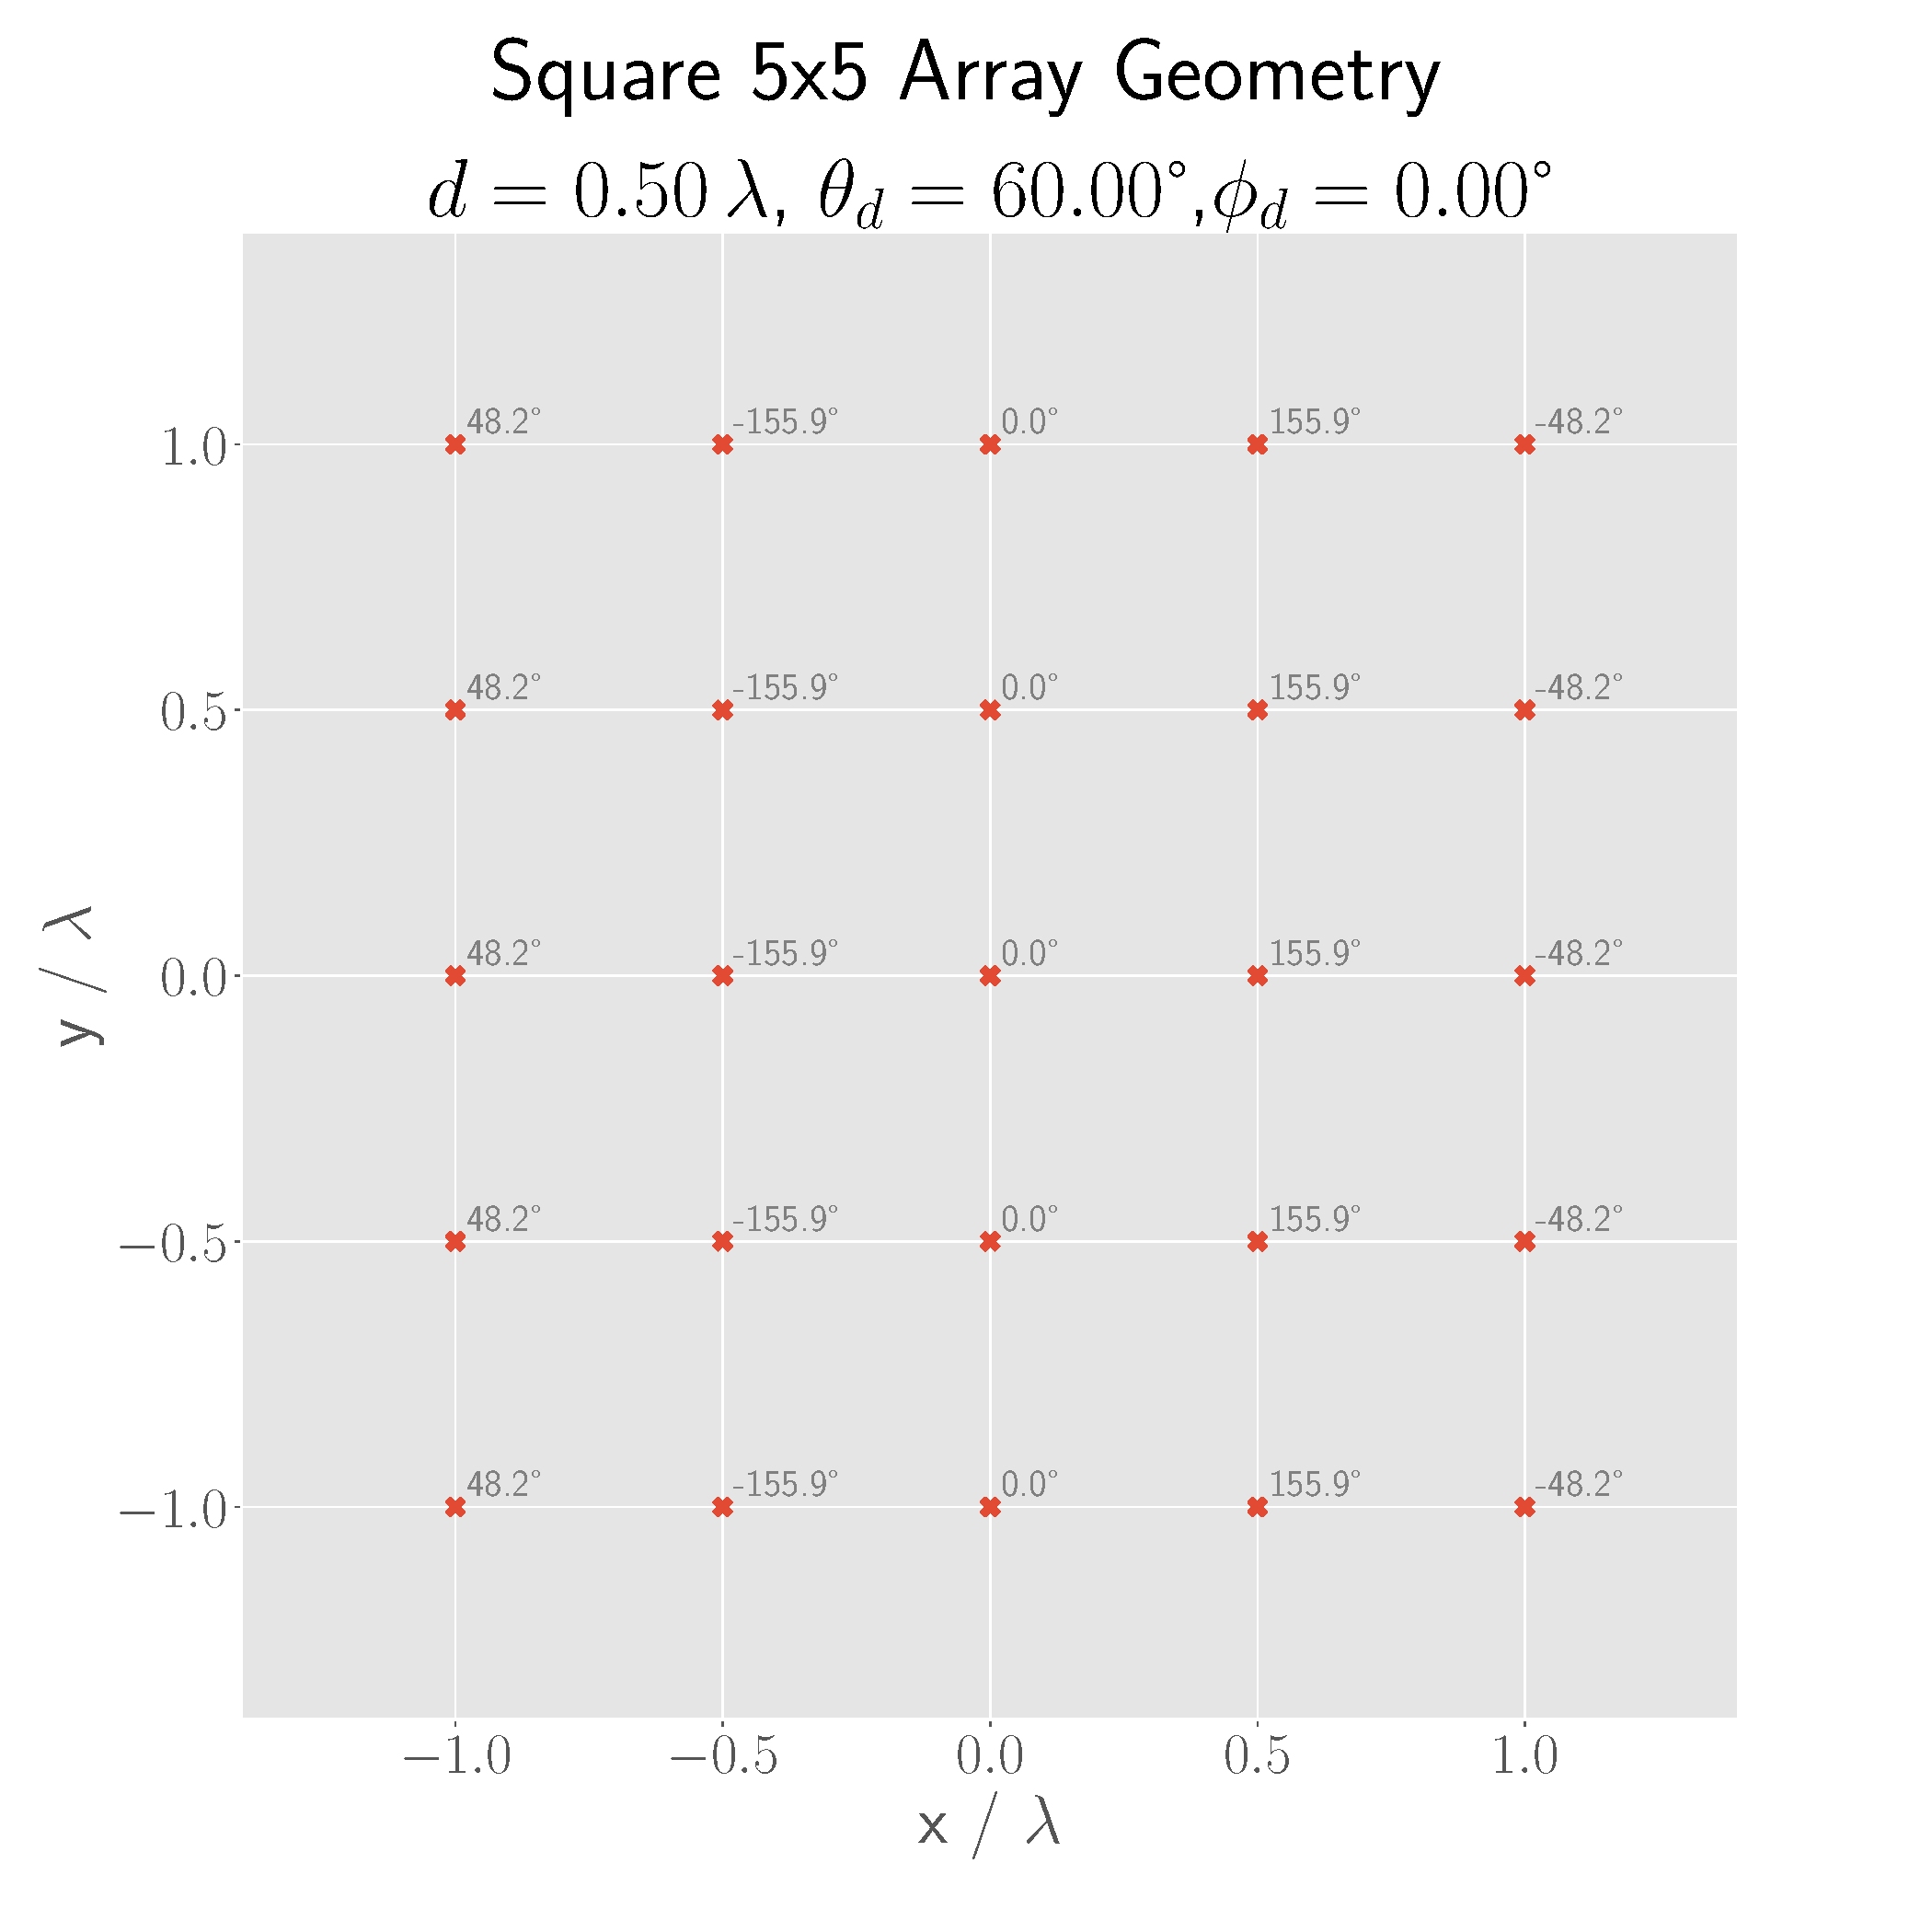
\includegraphics[width=\textwidth]{graphics/task_2/square-0.50-lambda-60.00-theta-0.00-phi-geometry.pdf}
    \caption{Square 5x5 Geometry with steering phases for $0.5\lambda$ spacing.}\label{fig:phase1}
  \end{minipage}\hfill
  \begin{minipage}[t]{0.45\textwidth}
    \centering
    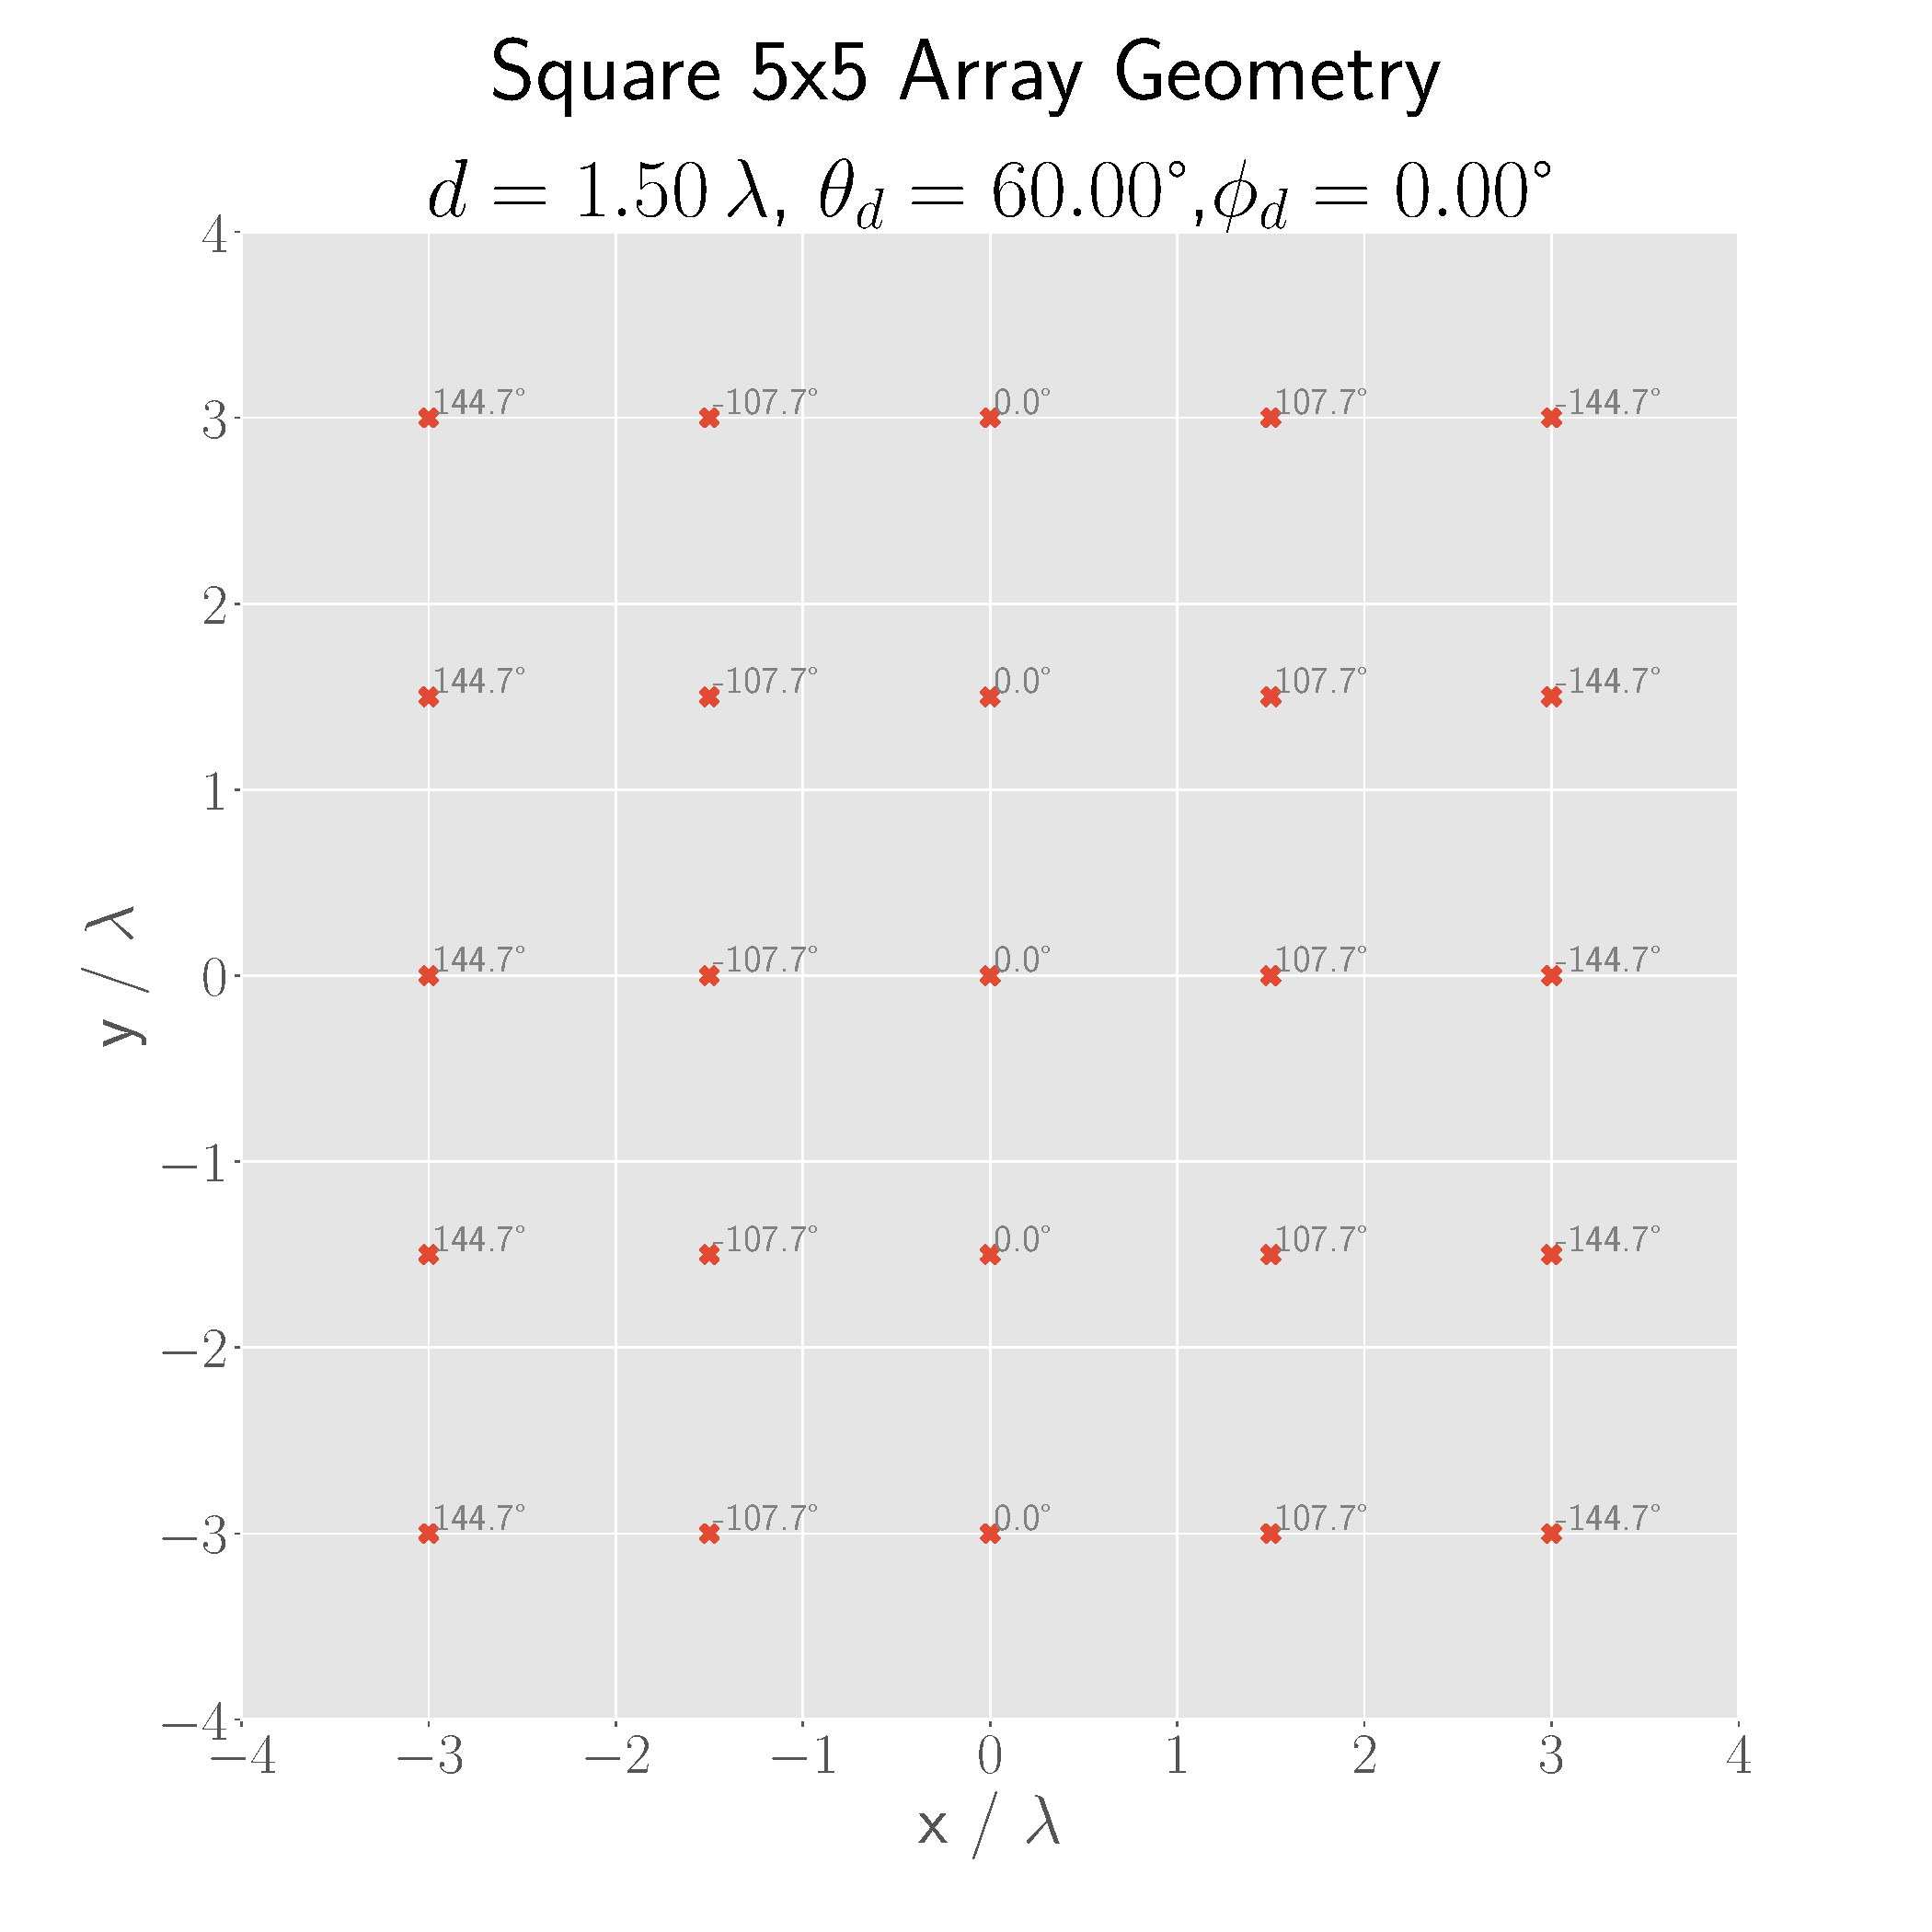
\includegraphics[width=\textwidth]{graphics/task_2/square-1.50-lambda-60.00-theta-0.00-phi-geometry.pdf}
    \caption{Square 5x5 Geometry with steering phases for $1.5\lambda$ spacing.}\label{fig:phase2}
   \end{minipage}
\end{figure}


In figures \ref{fig:phase1} and \ref{fig:phase2}, the array geometries along with the individual steering phases are shown for a target position of $\theta_{d}=60\,\si{\degree}, \phi_{d}=0\,\si{\degree}$. You can see that the phases are constant along the columns since any incident wave from a far-away target will have the same time of arrival for these antennas. Comparing the different spacings, the angle differences in the $d=1.5\lambda$ case are greater, which makes sense since their spacing is larger which results in more time lag.



\section{Equilateral Array}

The same figures have been generated for a 25-antenna array where the spacings were still equal but the grid of antennas is made from equilateral triangles. This reduces the spacing between the rows but also enlargens the array towards the left and right. This ``squishing'' effect can also be seen in the radiation patterns. The geometry can be seen in figure \ref{fig:equilat-geometry}.\\

The same principle regarding the spacing, grating lobes and beamwidth as in the square array case applies. However, the grating lobes along the $u$-direction are farther away and so appear at a greater angle.

\begin{figure}[h]
    \centering
    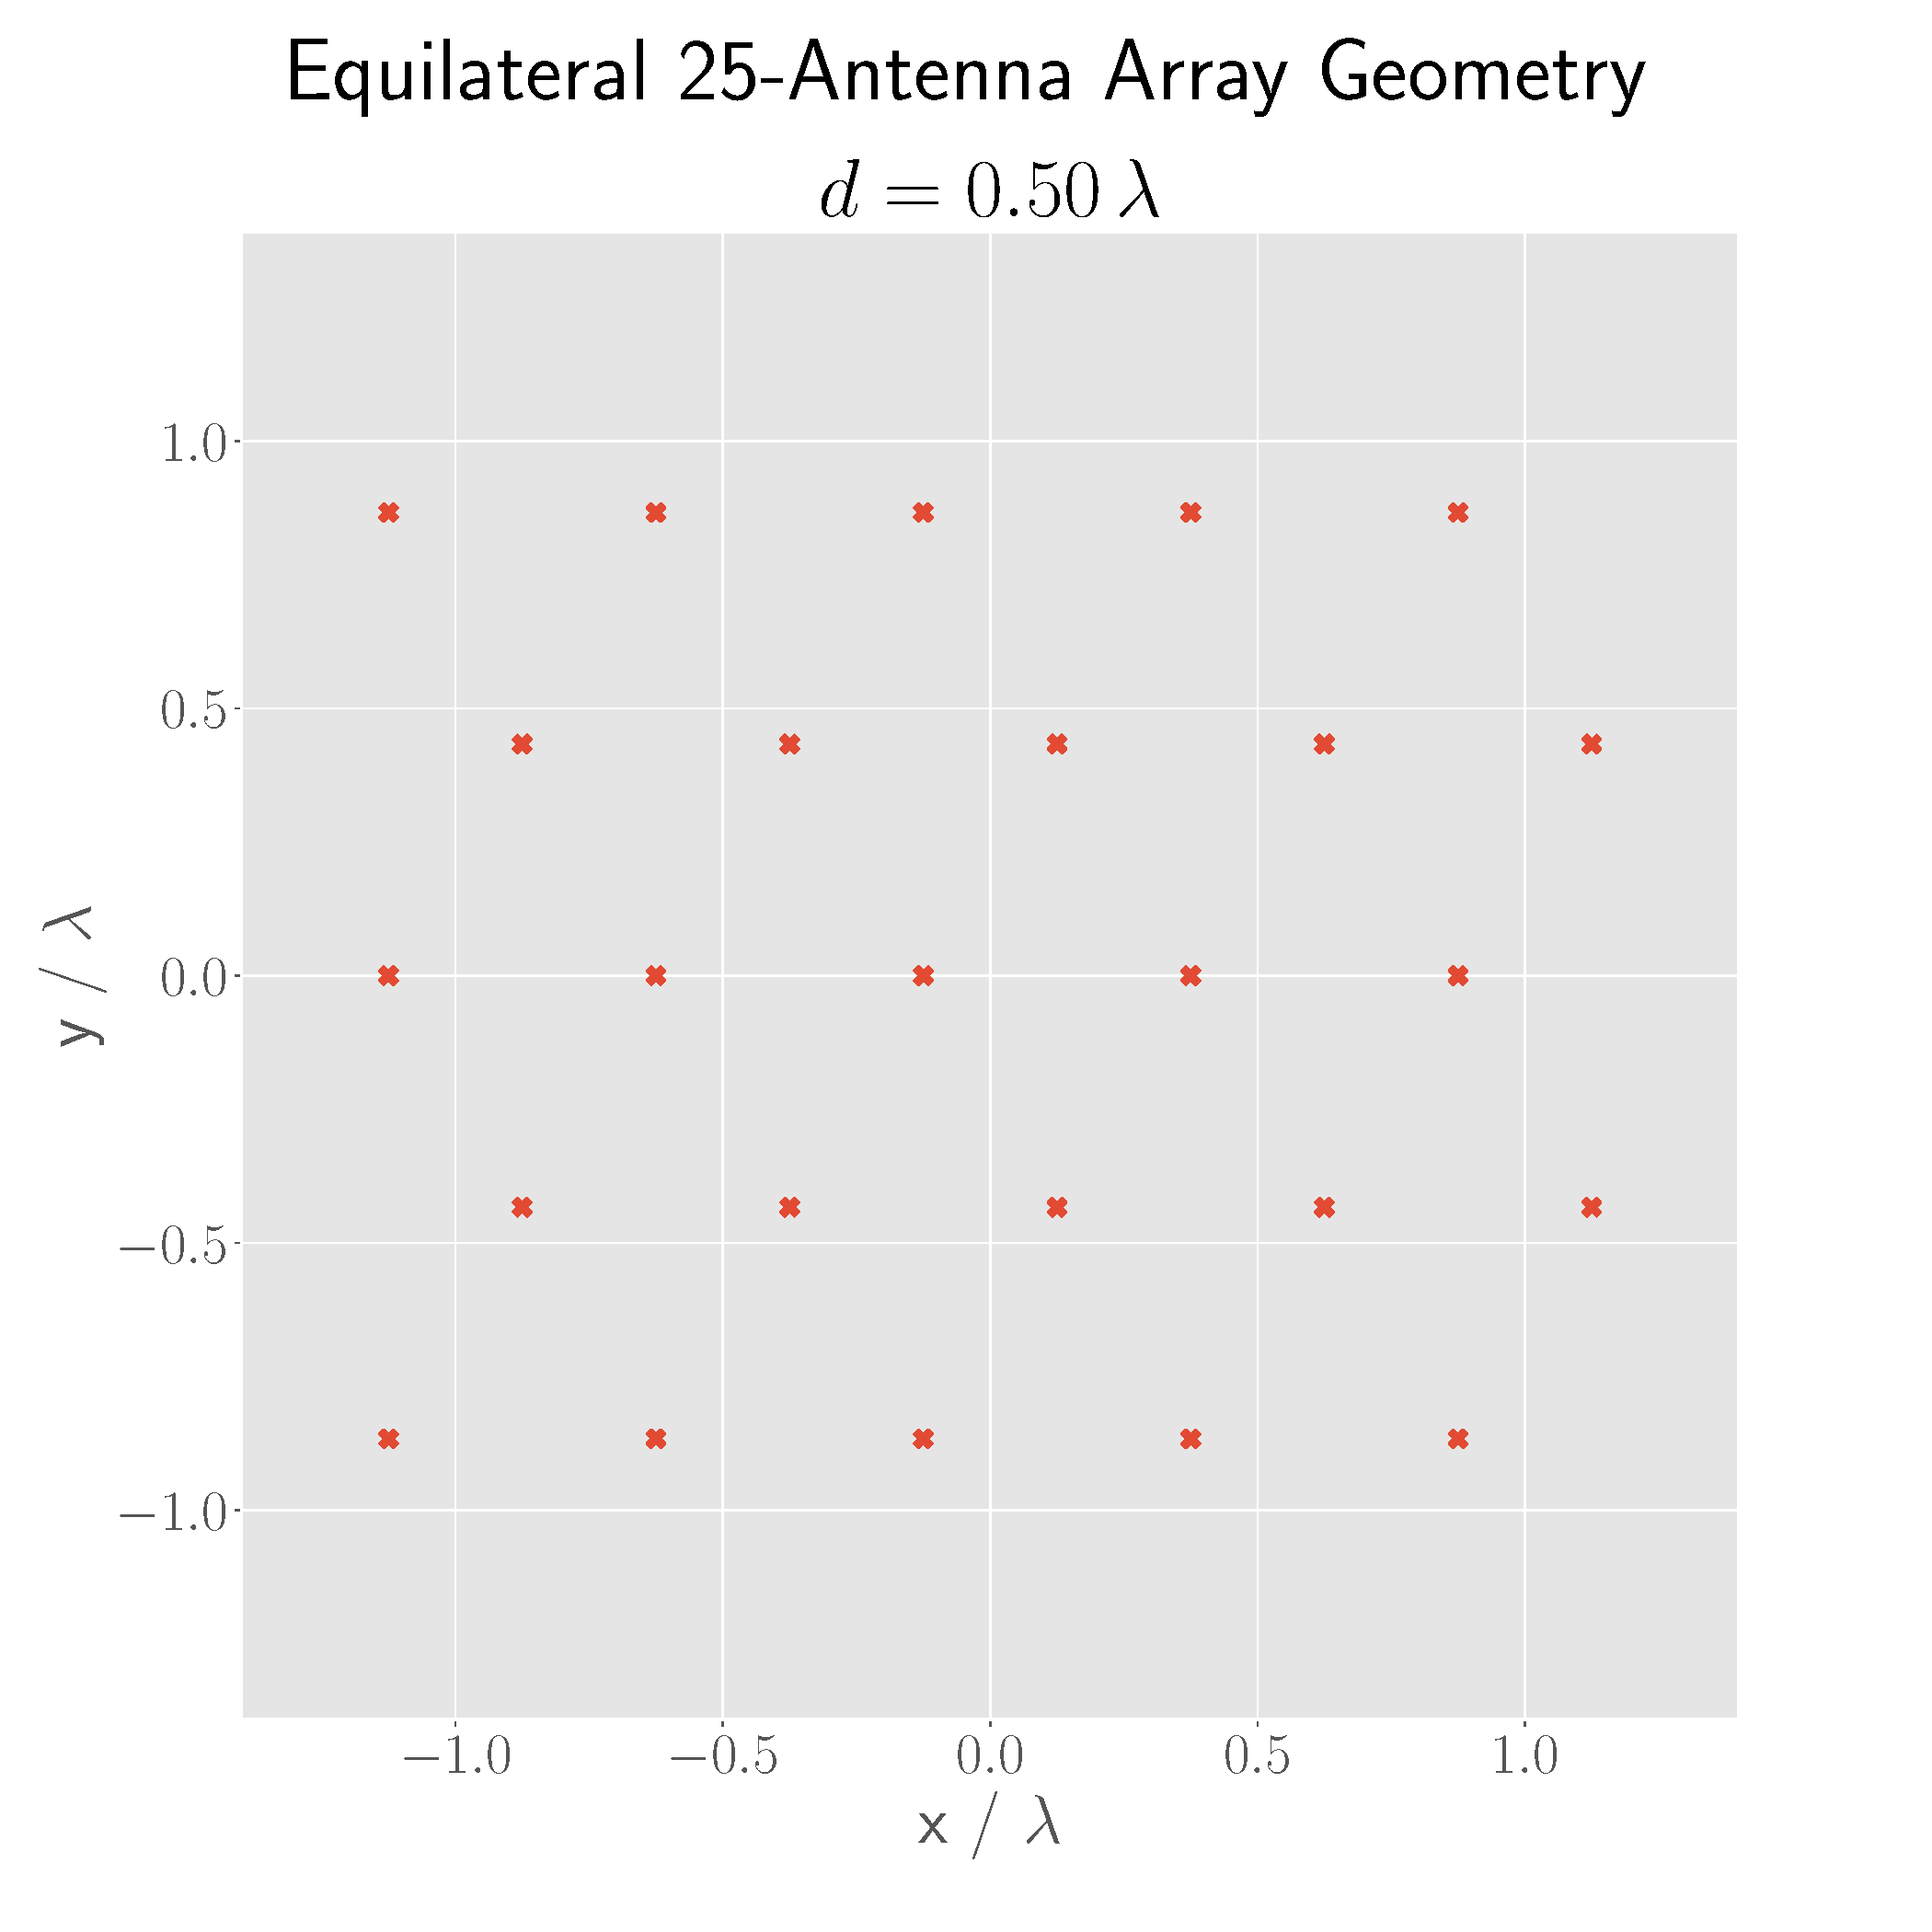
\includegraphics[width=0.4\textwidth]{graphics/task_3/equilat-0.50-lambda-0.00-theta-0.00-phi-geometry.pdf}
    \caption{Equilateral grid array structure for $d=0.5\,\lambda$}\label{fig:equilat-geometry}
\end{figure}

\begin{figure}[H]
  \begin{minipage}[t]{0.45\textwidth}
    \centering
    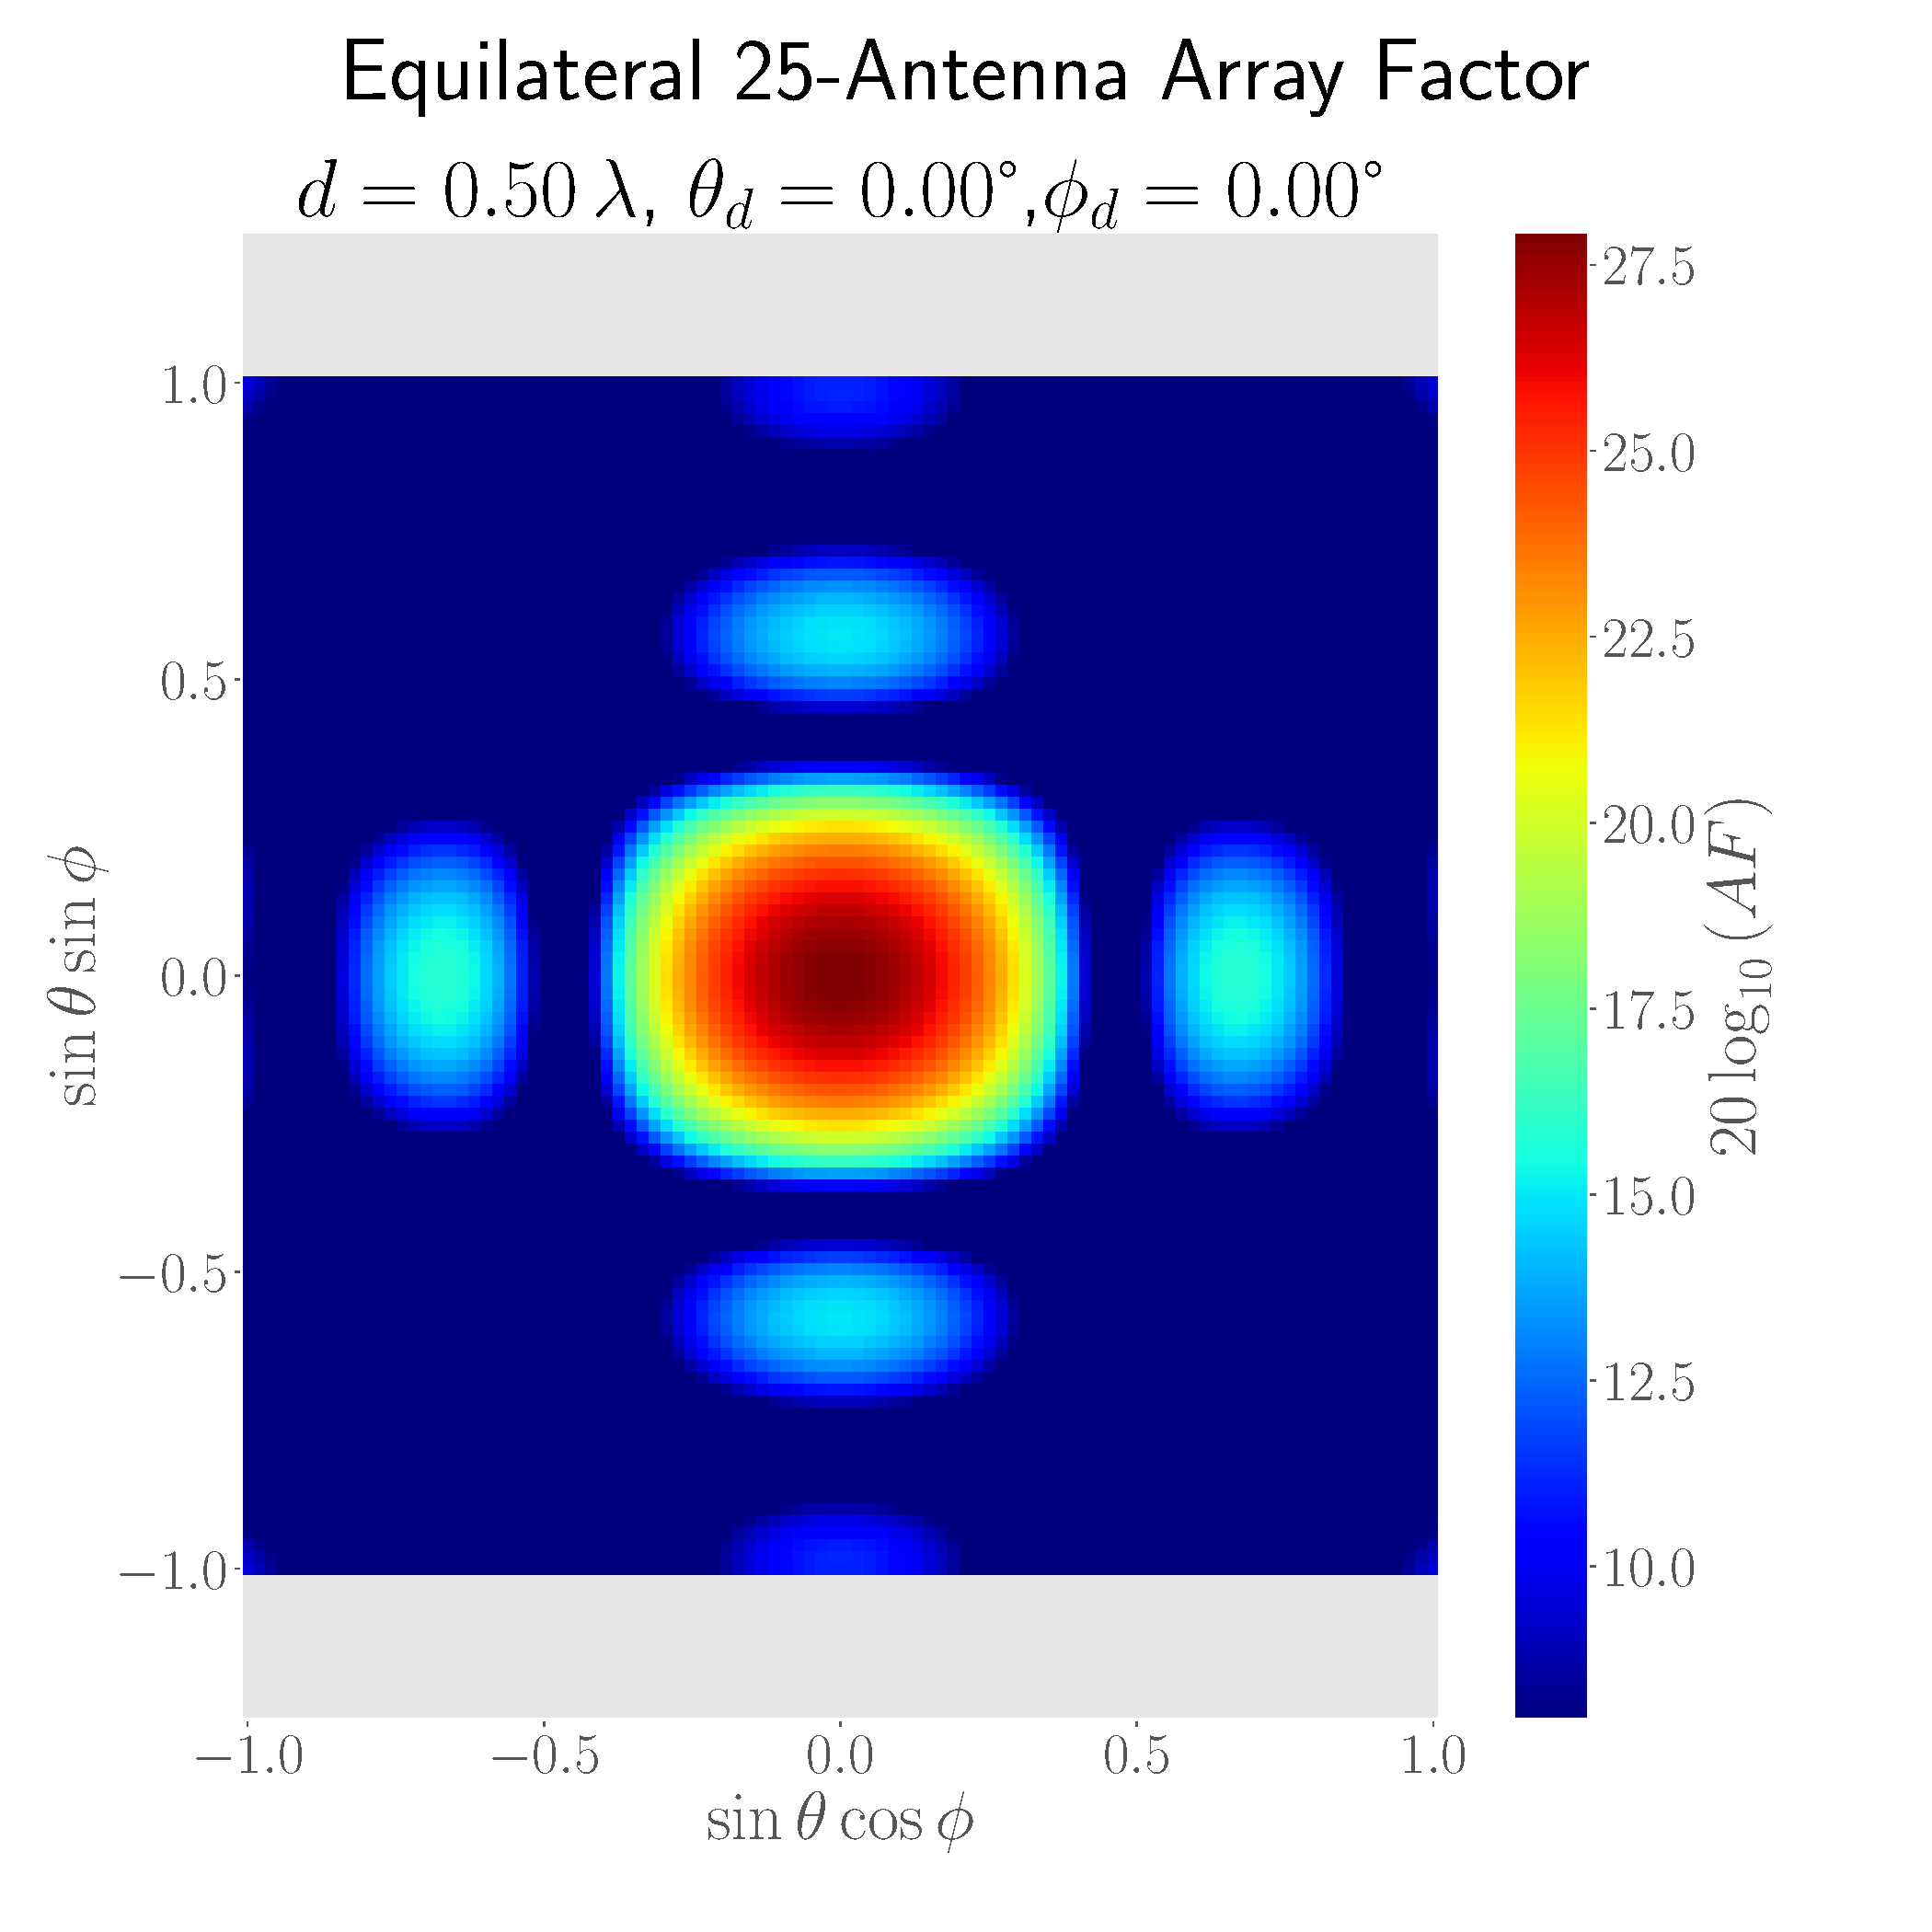
\includegraphics[width=\textwidth]{graphics/task_3/equilat-0.50-lambda-0.00-theta-0.00-phi-radpat.pdf}
    \caption{Equilateral vertically steered radiation pattern for $0.5\lambda$ spacing.}\label{fig:rad-equilat-0.5-0}
  \end{minipage}\hfill
  \begin{minipage}[t]{0.45\textwidth}
    \centering
    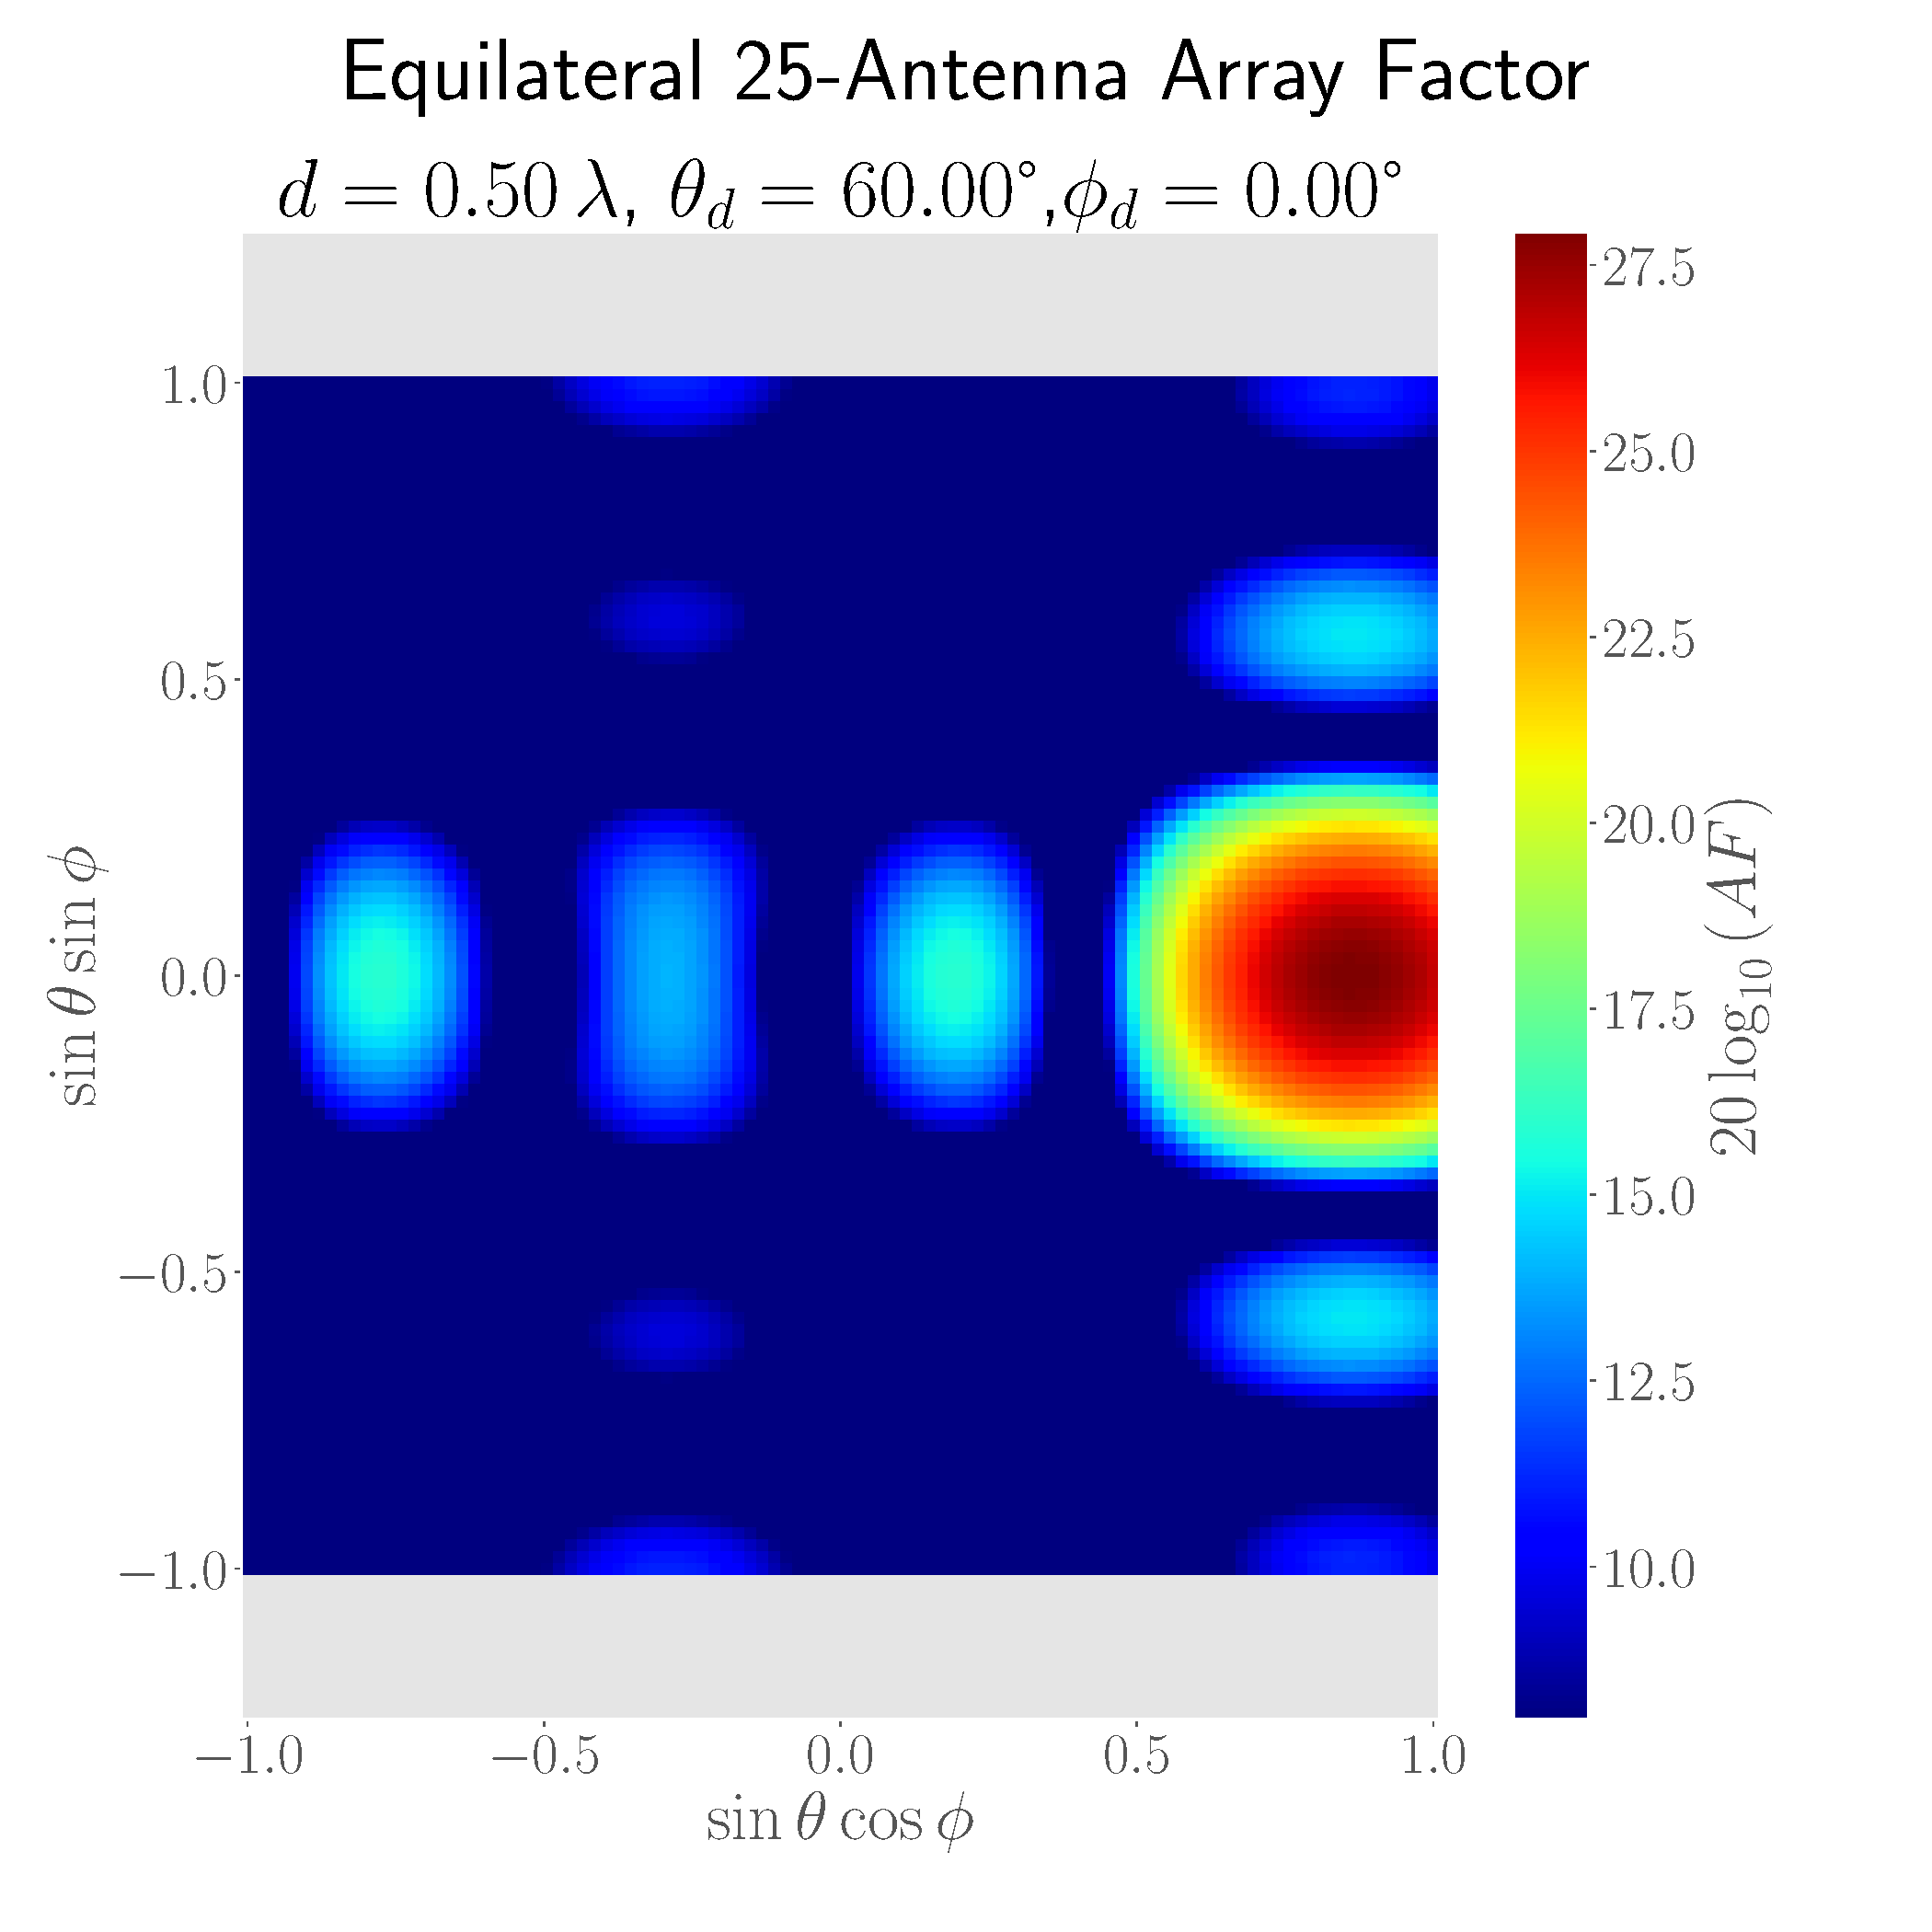
\includegraphics[width=\textwidth]{graphics/task_3/equilat-0.50-lambda-60.00-theta-0.00-phi-radpat.pdf}
    \caption{Equilateral off-vertically steered radiation pattern for $0.5\lambda$ spacing.}\label{fig:rad-equilat-0.5-60}
   \end{minipage}
\end{figure}

\begin{figure}[H]
  \begin{minipage}[t]{0.45\textwidth}
    \centering
    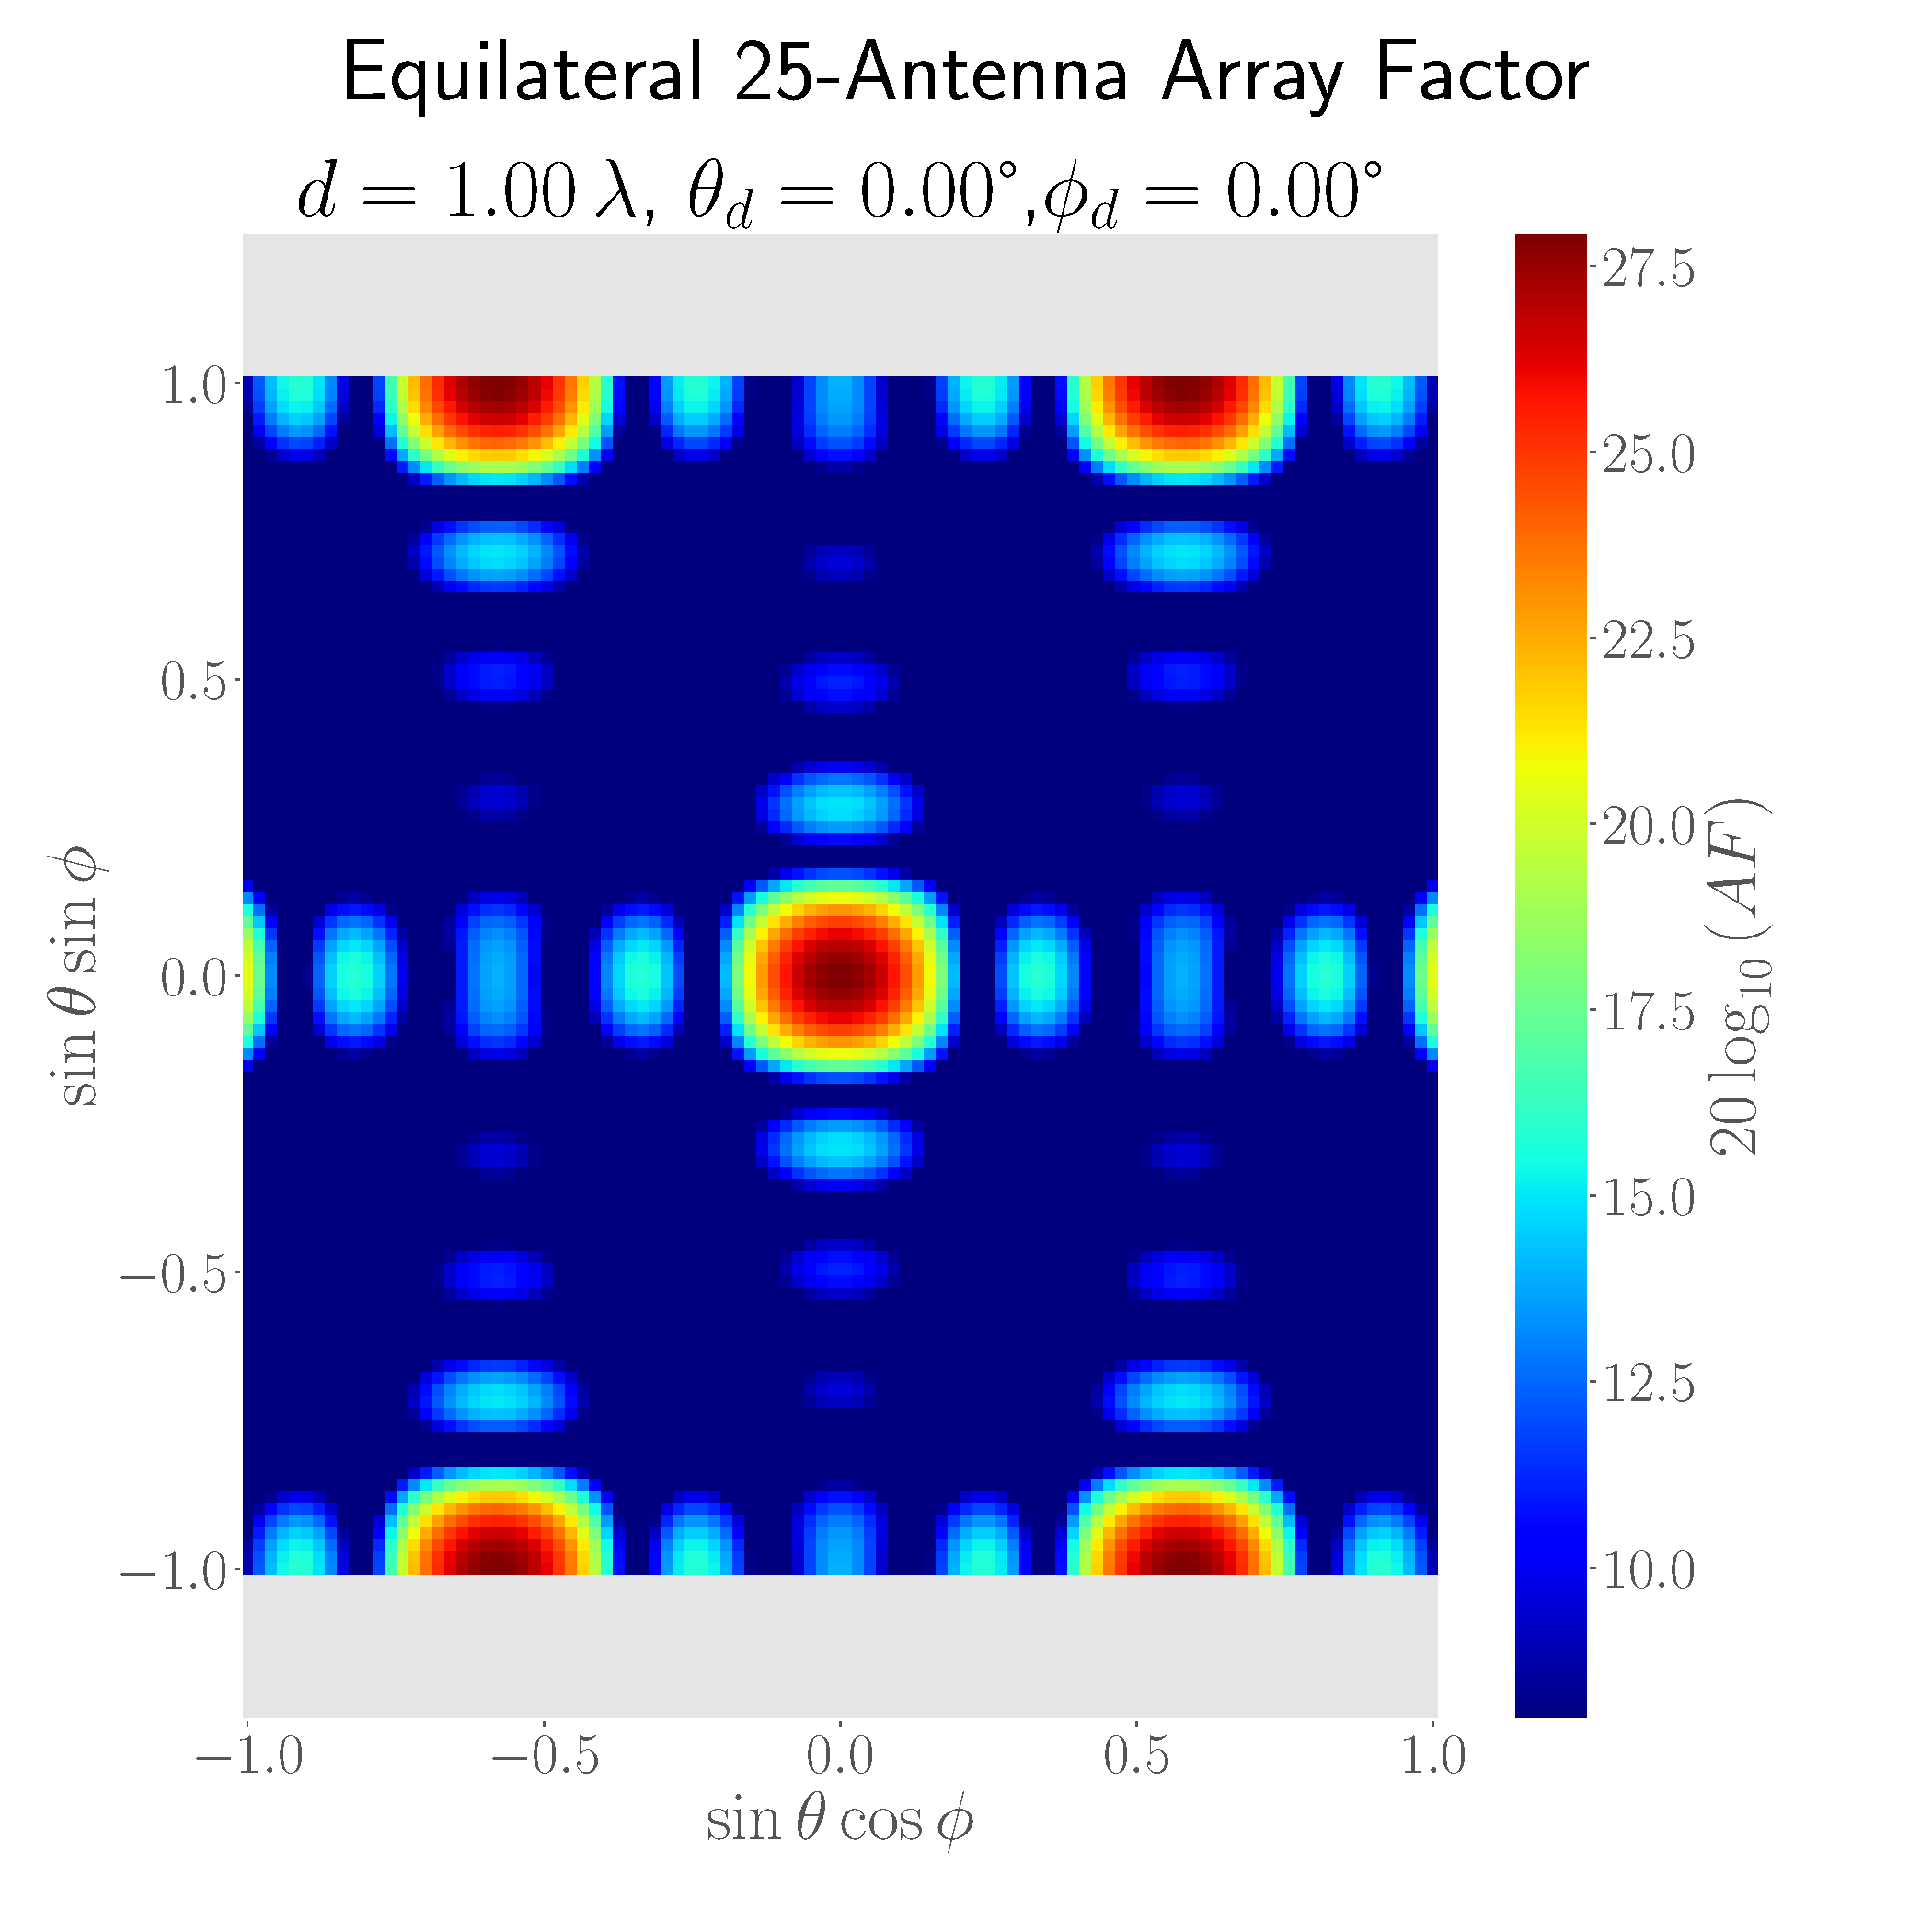
\includegraphics[width=\textwidth]{graphics/task_3/equilat-1.00-lambda-0.00-theta-0.00-phi-radpat.pdf}
    \caption{Equilateral vertically steered radiation pattern for $1.0\lambda$ spacing.}\label{fig:rad-equilat-1.0-0}
  \end{minipage}\hfill
  \begin{minipage}[t]{0.45\textwidth}
    \centering
    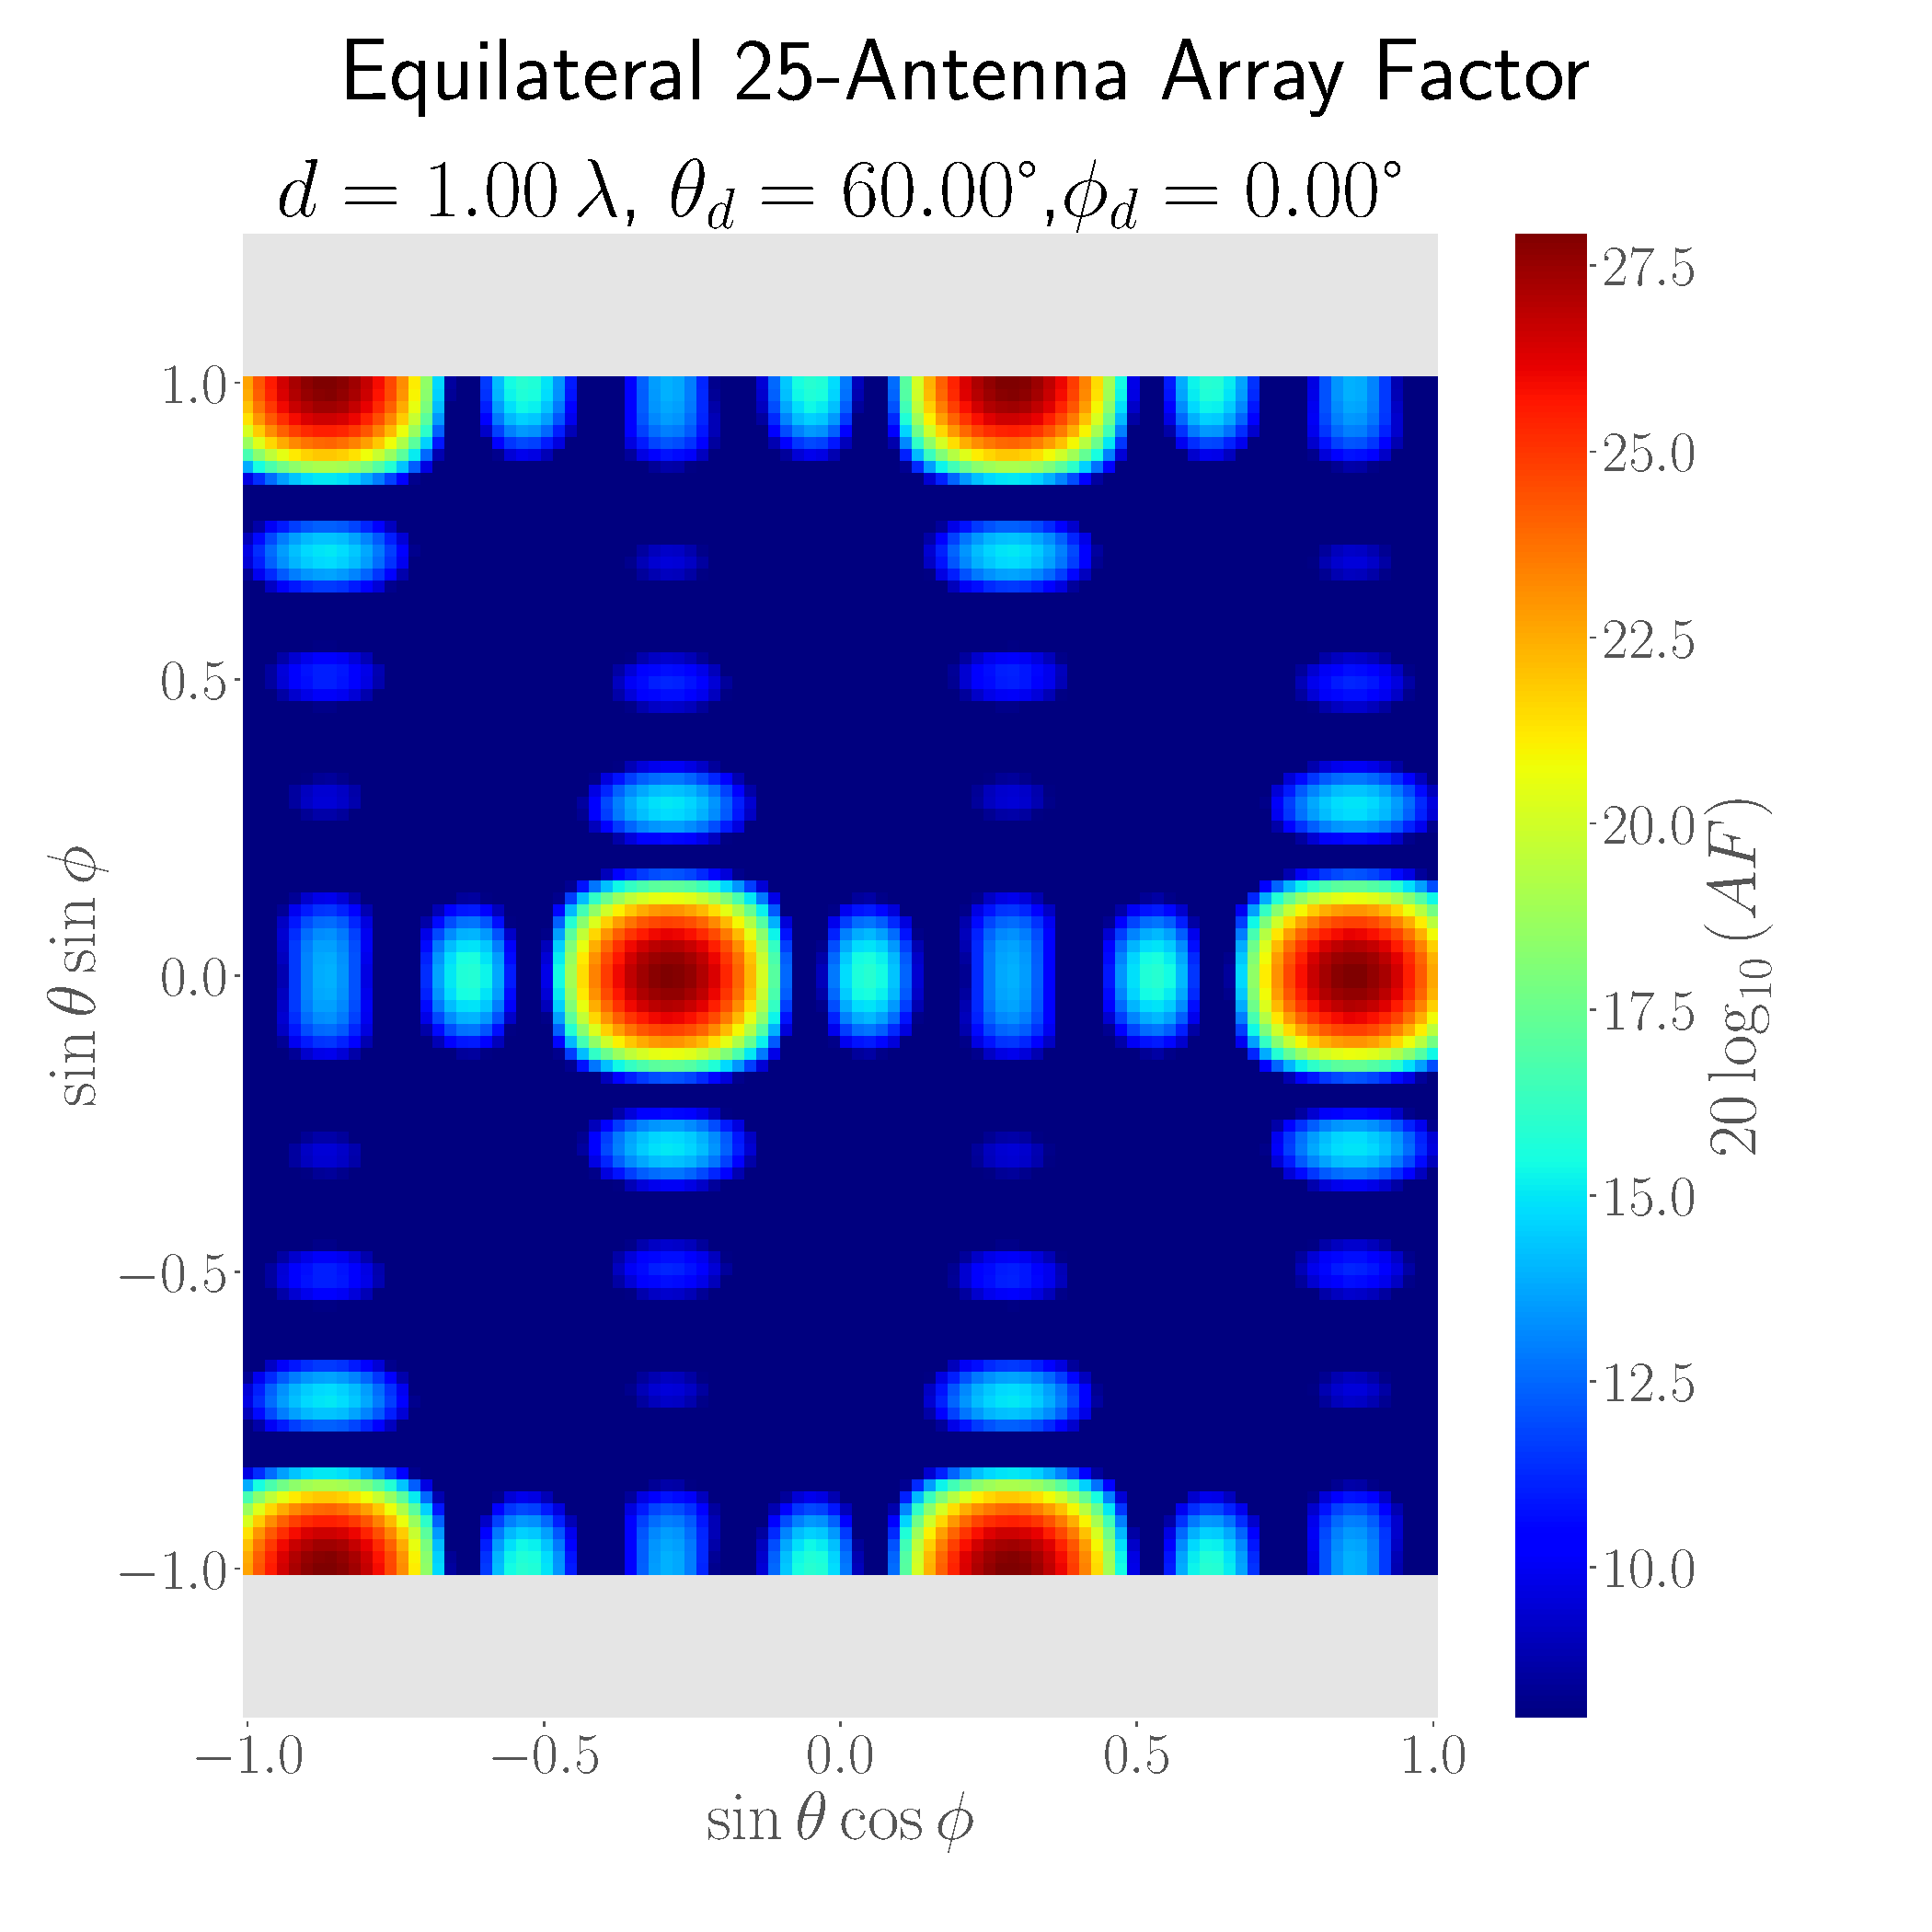
\includegraphics[width=\textwidth]{graphics/task_3/equilat-1.00-lambda-60.00-theta-0.00-phi-radpat.pdf}
    \caption{Equilateral off-vertically steered radiation pattern for $1.0\lambda$ spacing.}\label{fig:rad-equilat-1.0-60}
   \end{minipage}
\end{figure}

\begin{figure}[H]
  \begin{minipage}[t]{0.45\textwidth}
    \centering
    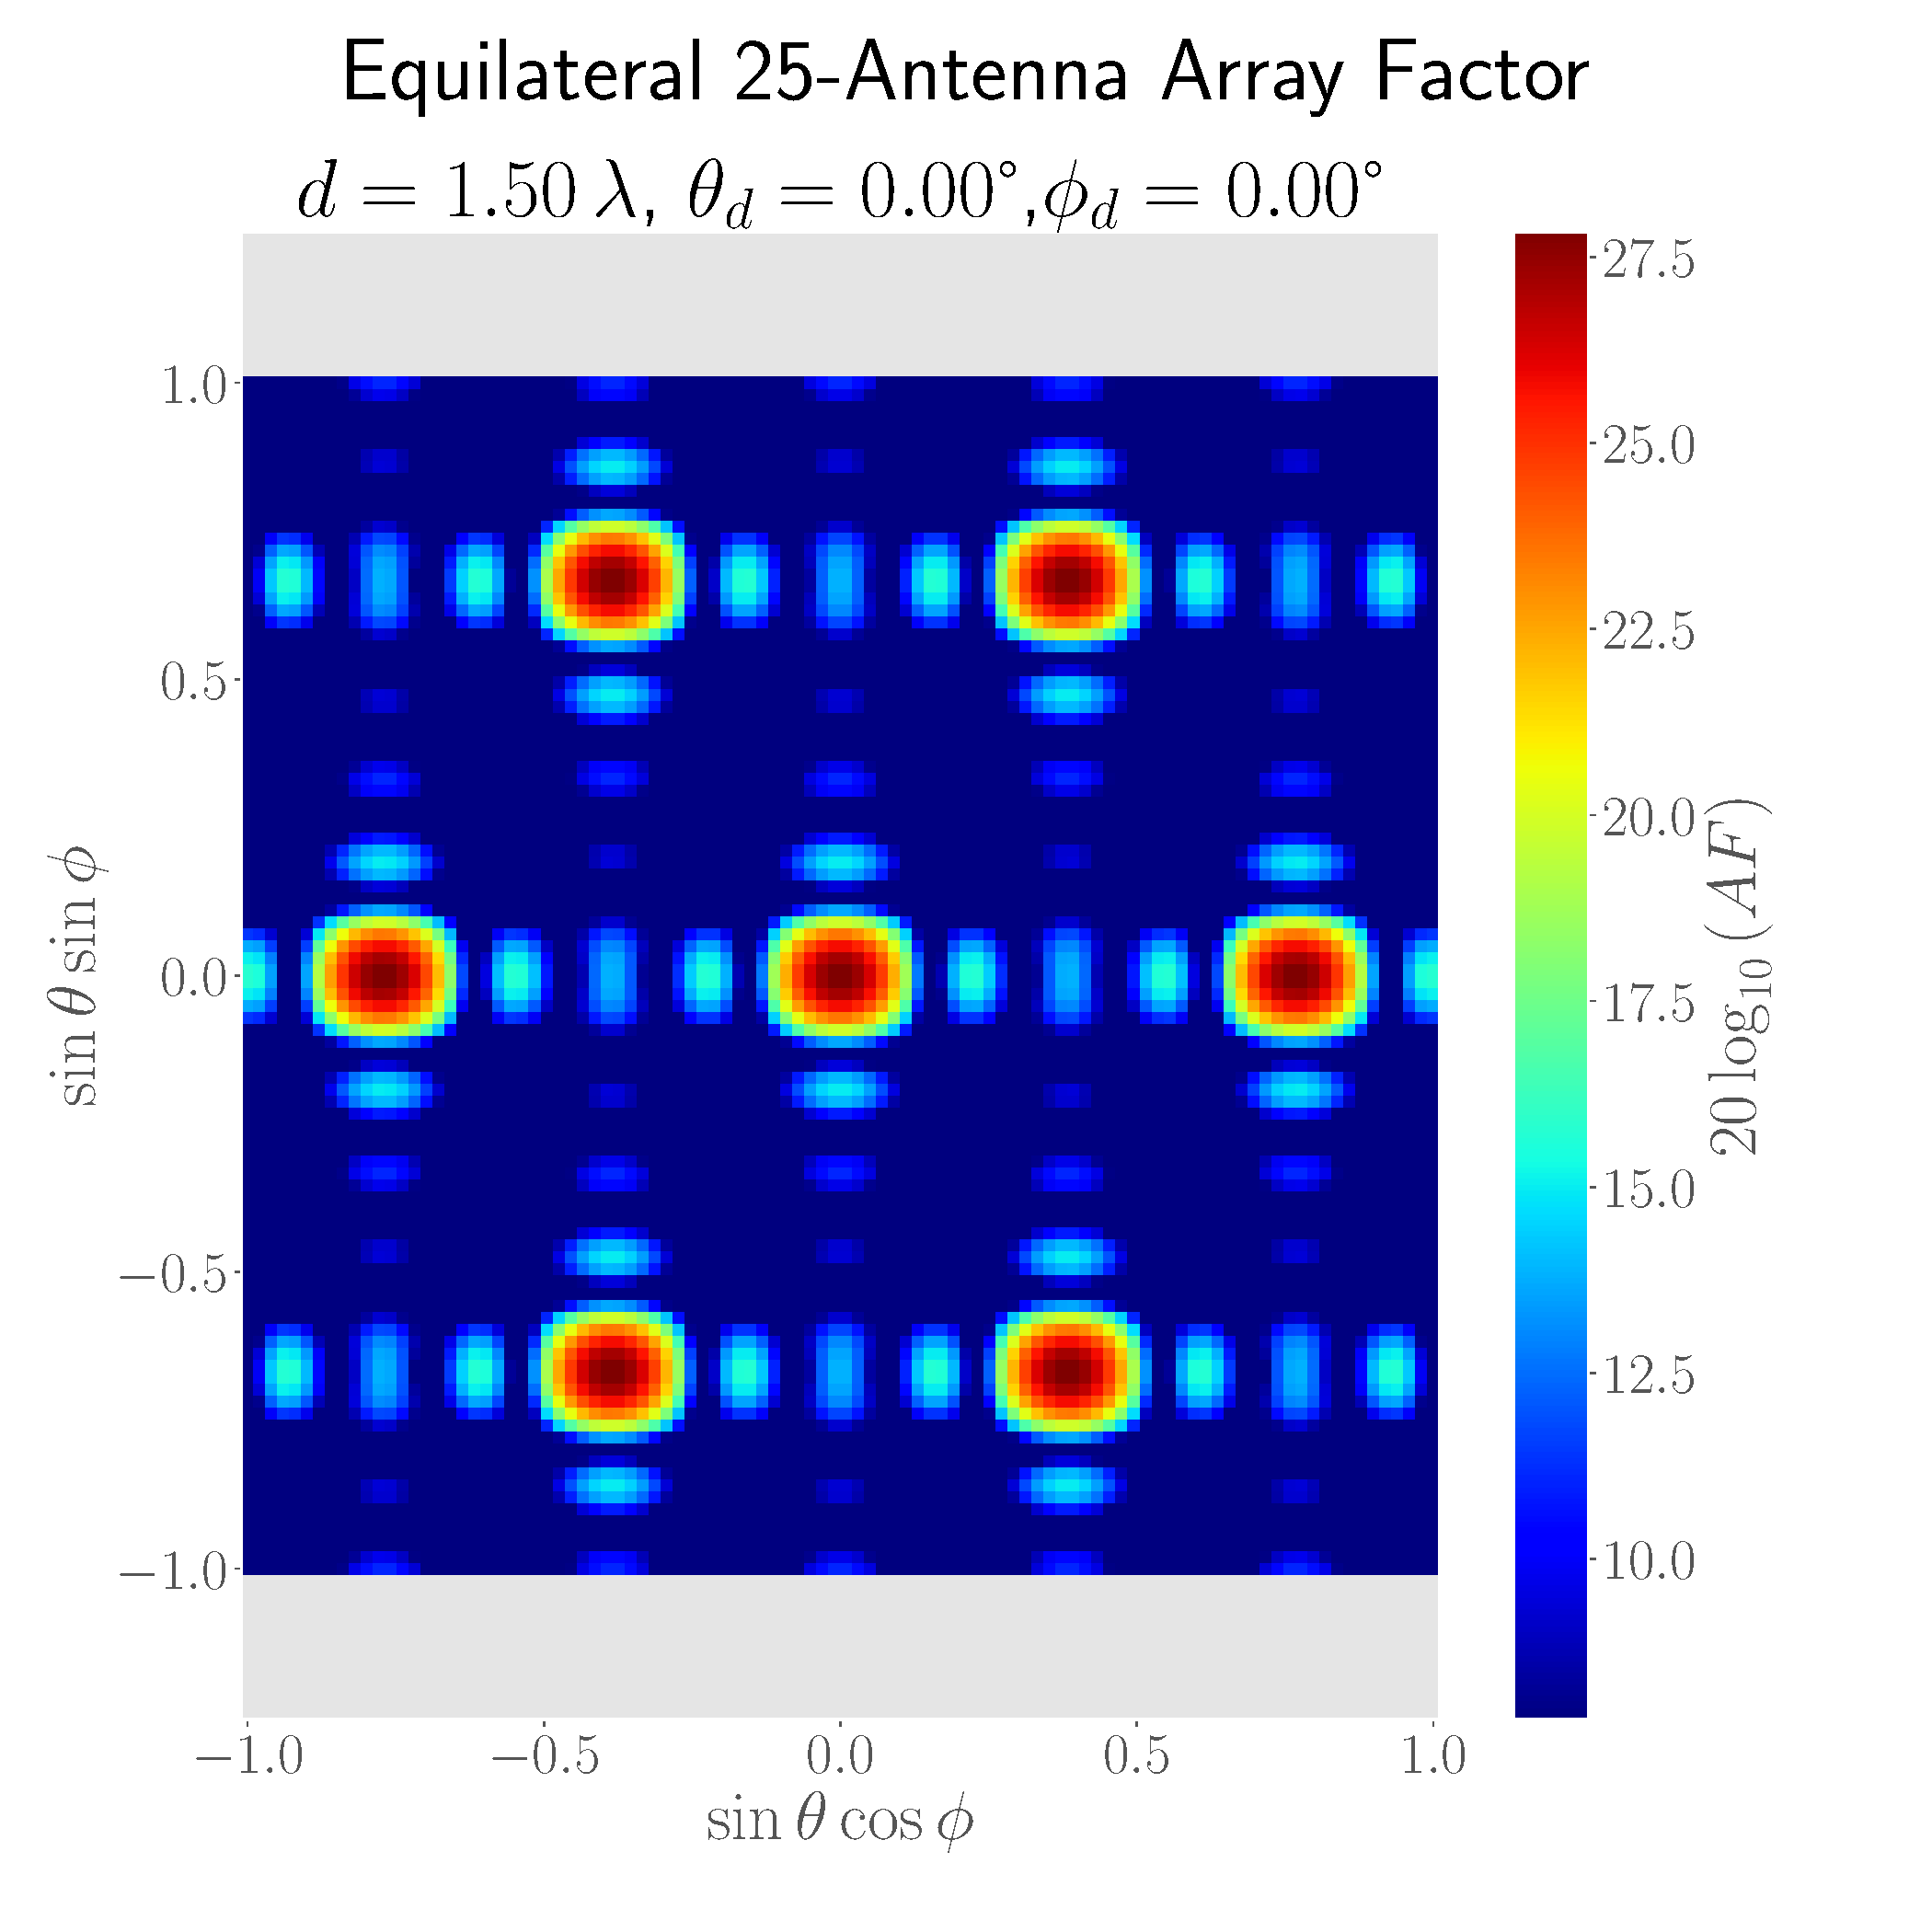
\includegraphics[width=\textwidth]{graphics/task_3/equilat-1.50-lambda-0.00-theta-0.00-phi-radpat.pdf}
    \caption{Equilateral vertically steered radiation pattern for $1.5\lambda$ spacing.}\label{fig:rad-equilat-1.5-0}
  \end{minipage}\hfill
  \begin{minipage}[t]{0.45\textwidth}
    \centering
    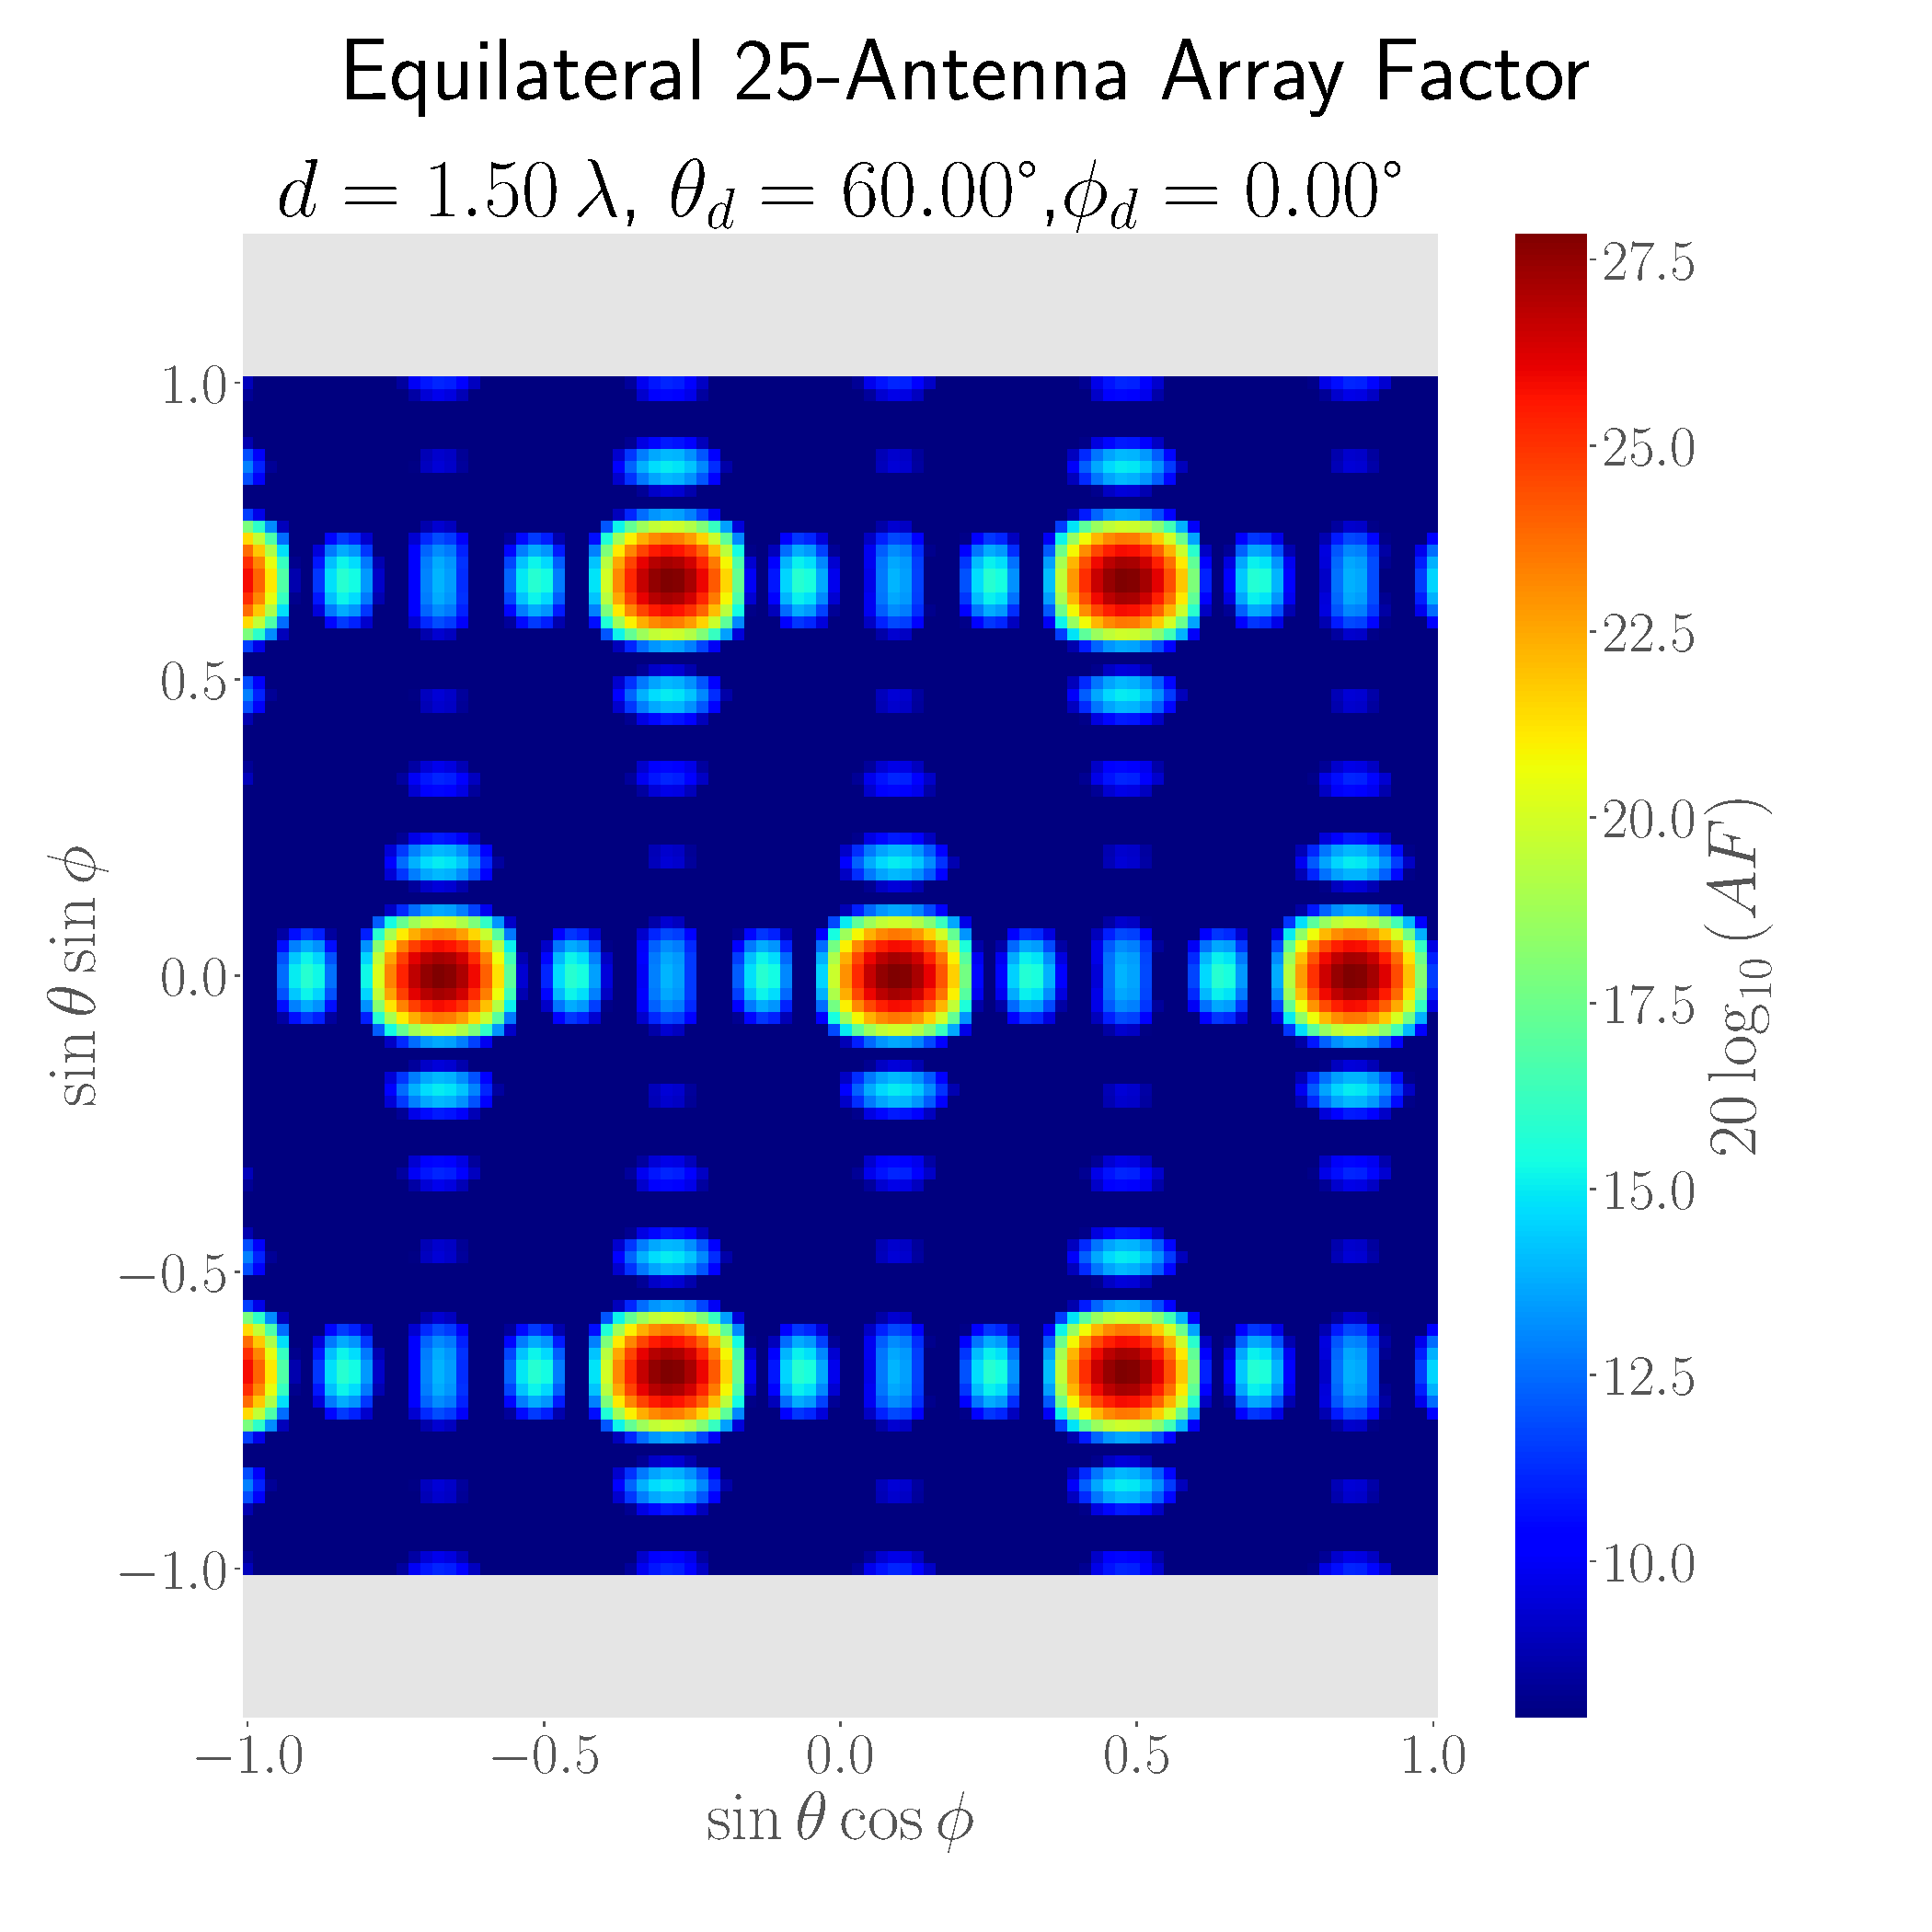
\includegraphics[width=\textwidth]{graphics/task_3/equilat-1.50-lambda-60.00-theta-0.00-phi-radpat.pdf}
    \caption{Equilateral off-vertically steered radiation pattern for $1.5\lambda$ spacing.}\label{fig:rad-equilat-1.5-60}
   \end{minipage}
\end{figure}


\begin{figure}[h]
    \centering
    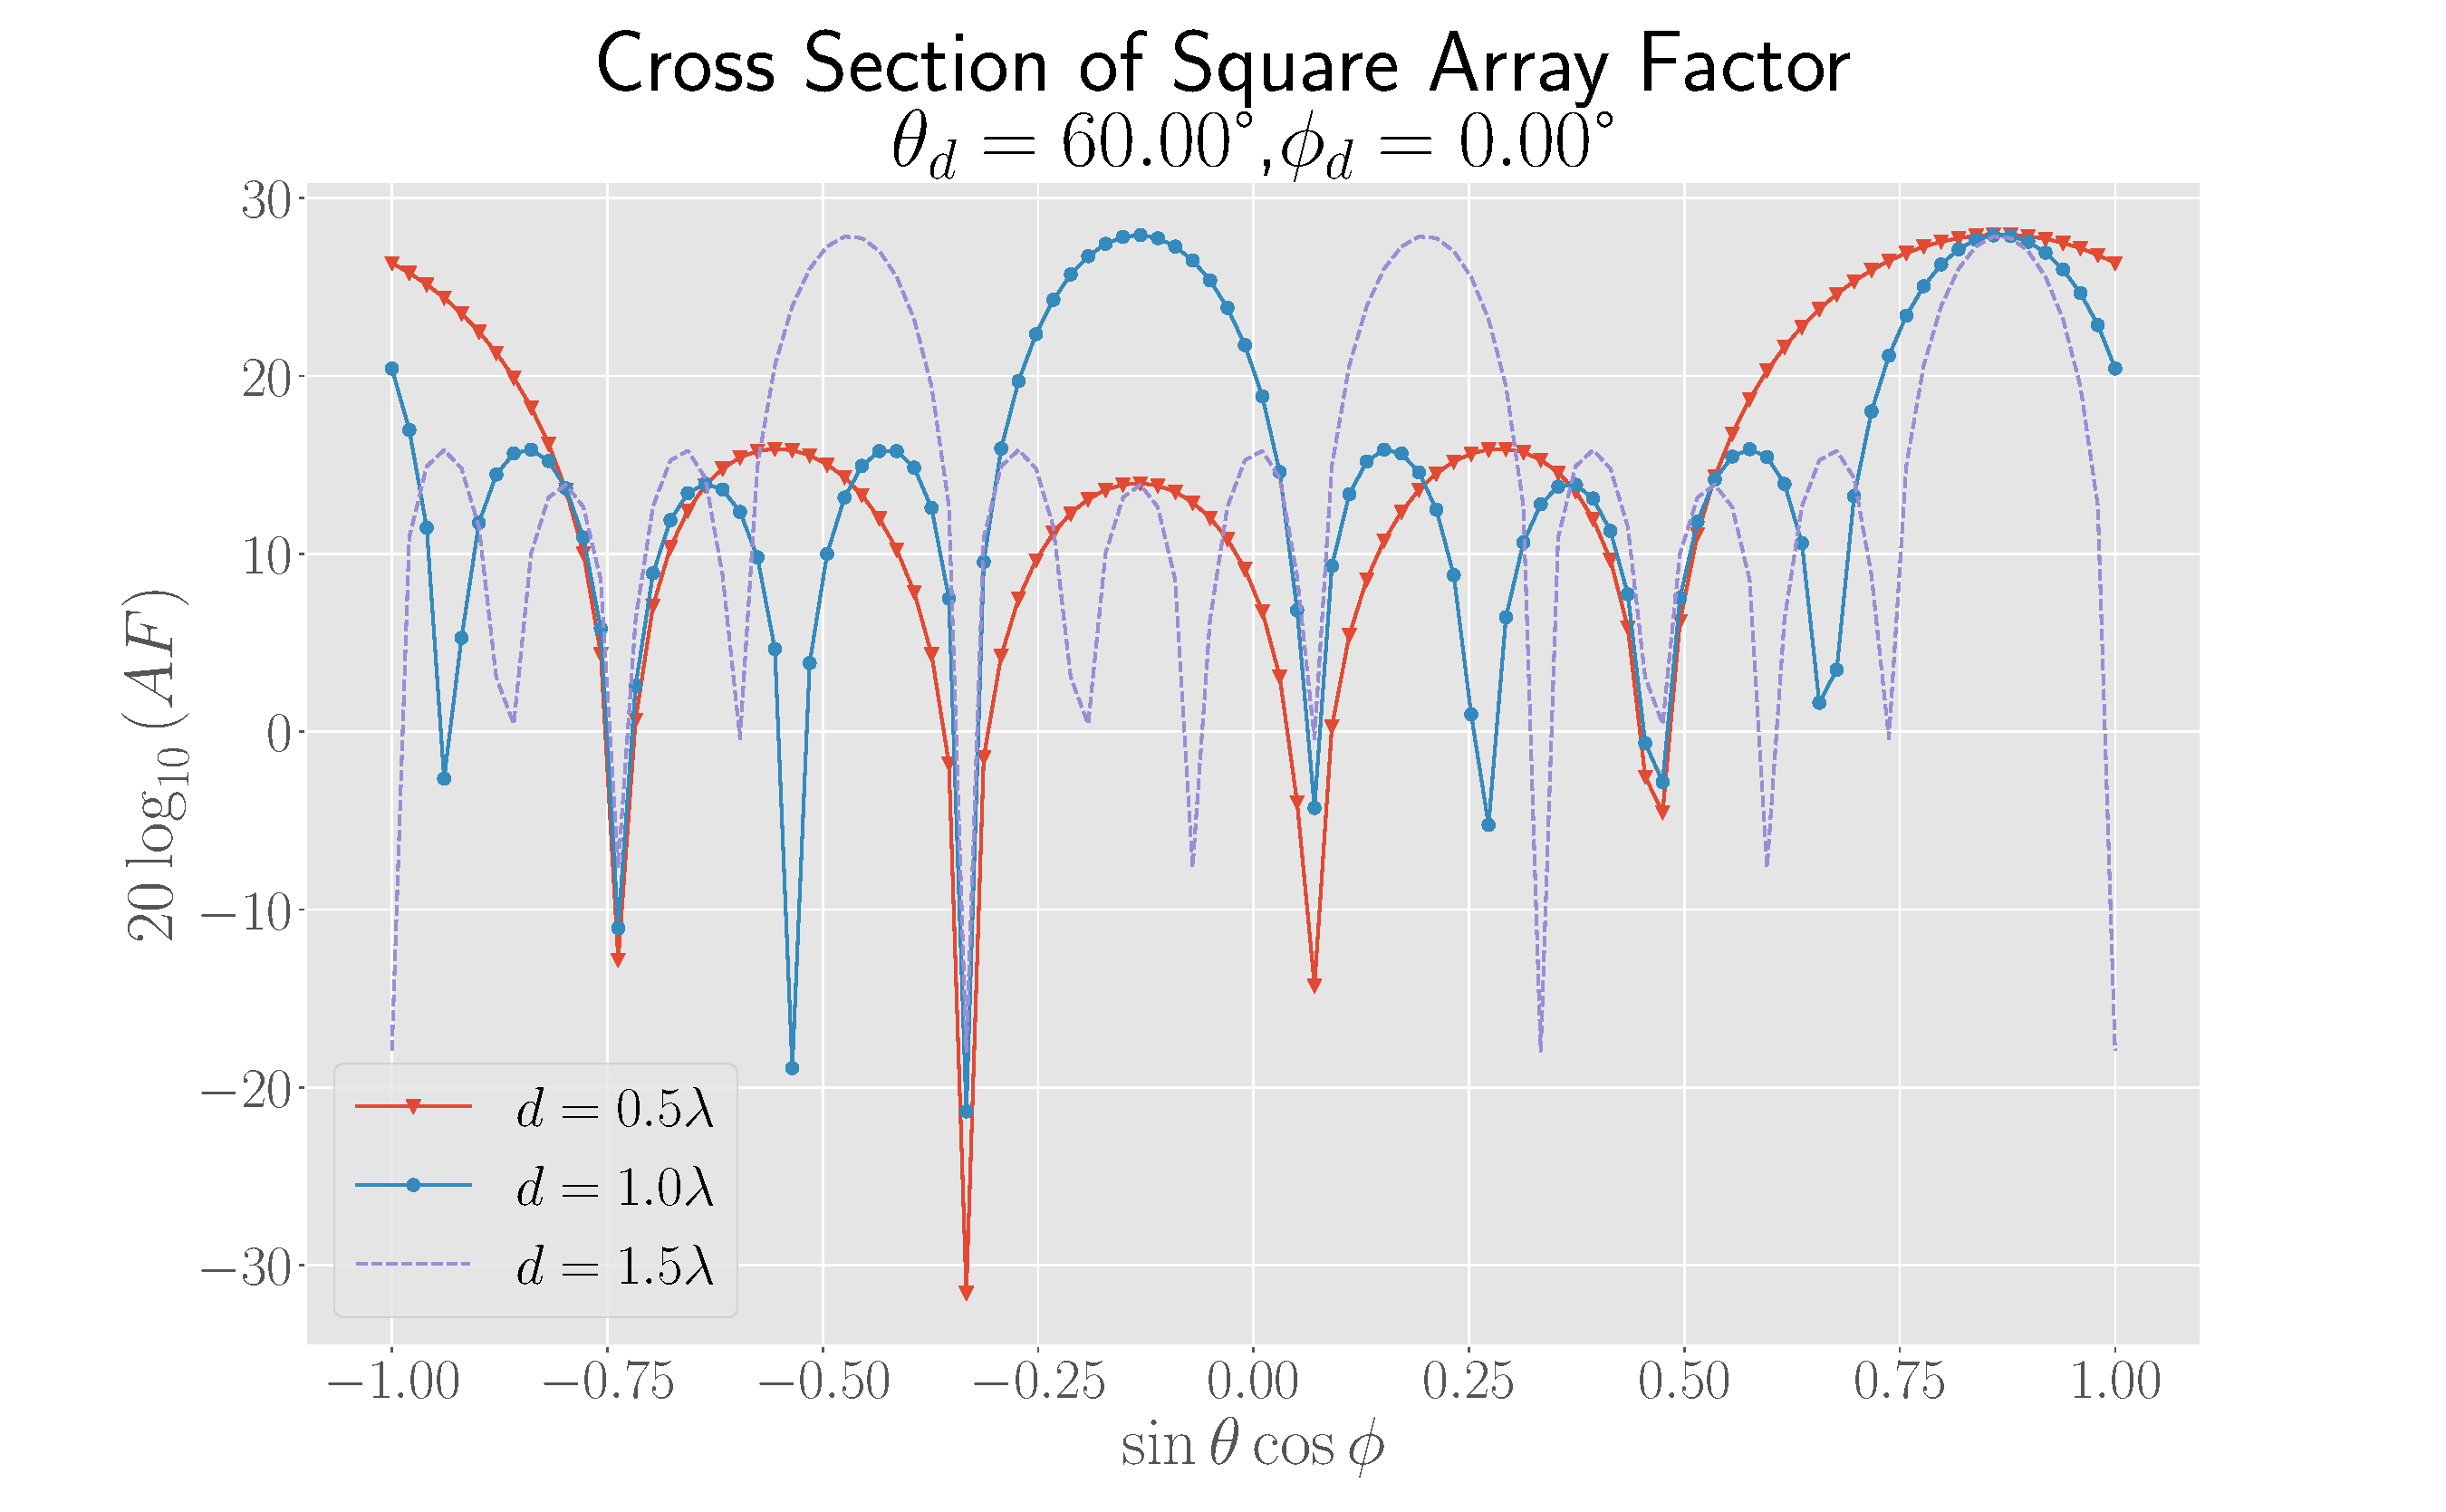
\includegraphics[width=0.618\textwidth]{graphics/task_1/square-60.00-theta-0.00-phi-cross.pdf}
    \caption{Comparison of cross-sections of the square array factor for different spacings.}\label{fig:square-cross}
\end{figure}


\begin{figure}[h]
    \centering
    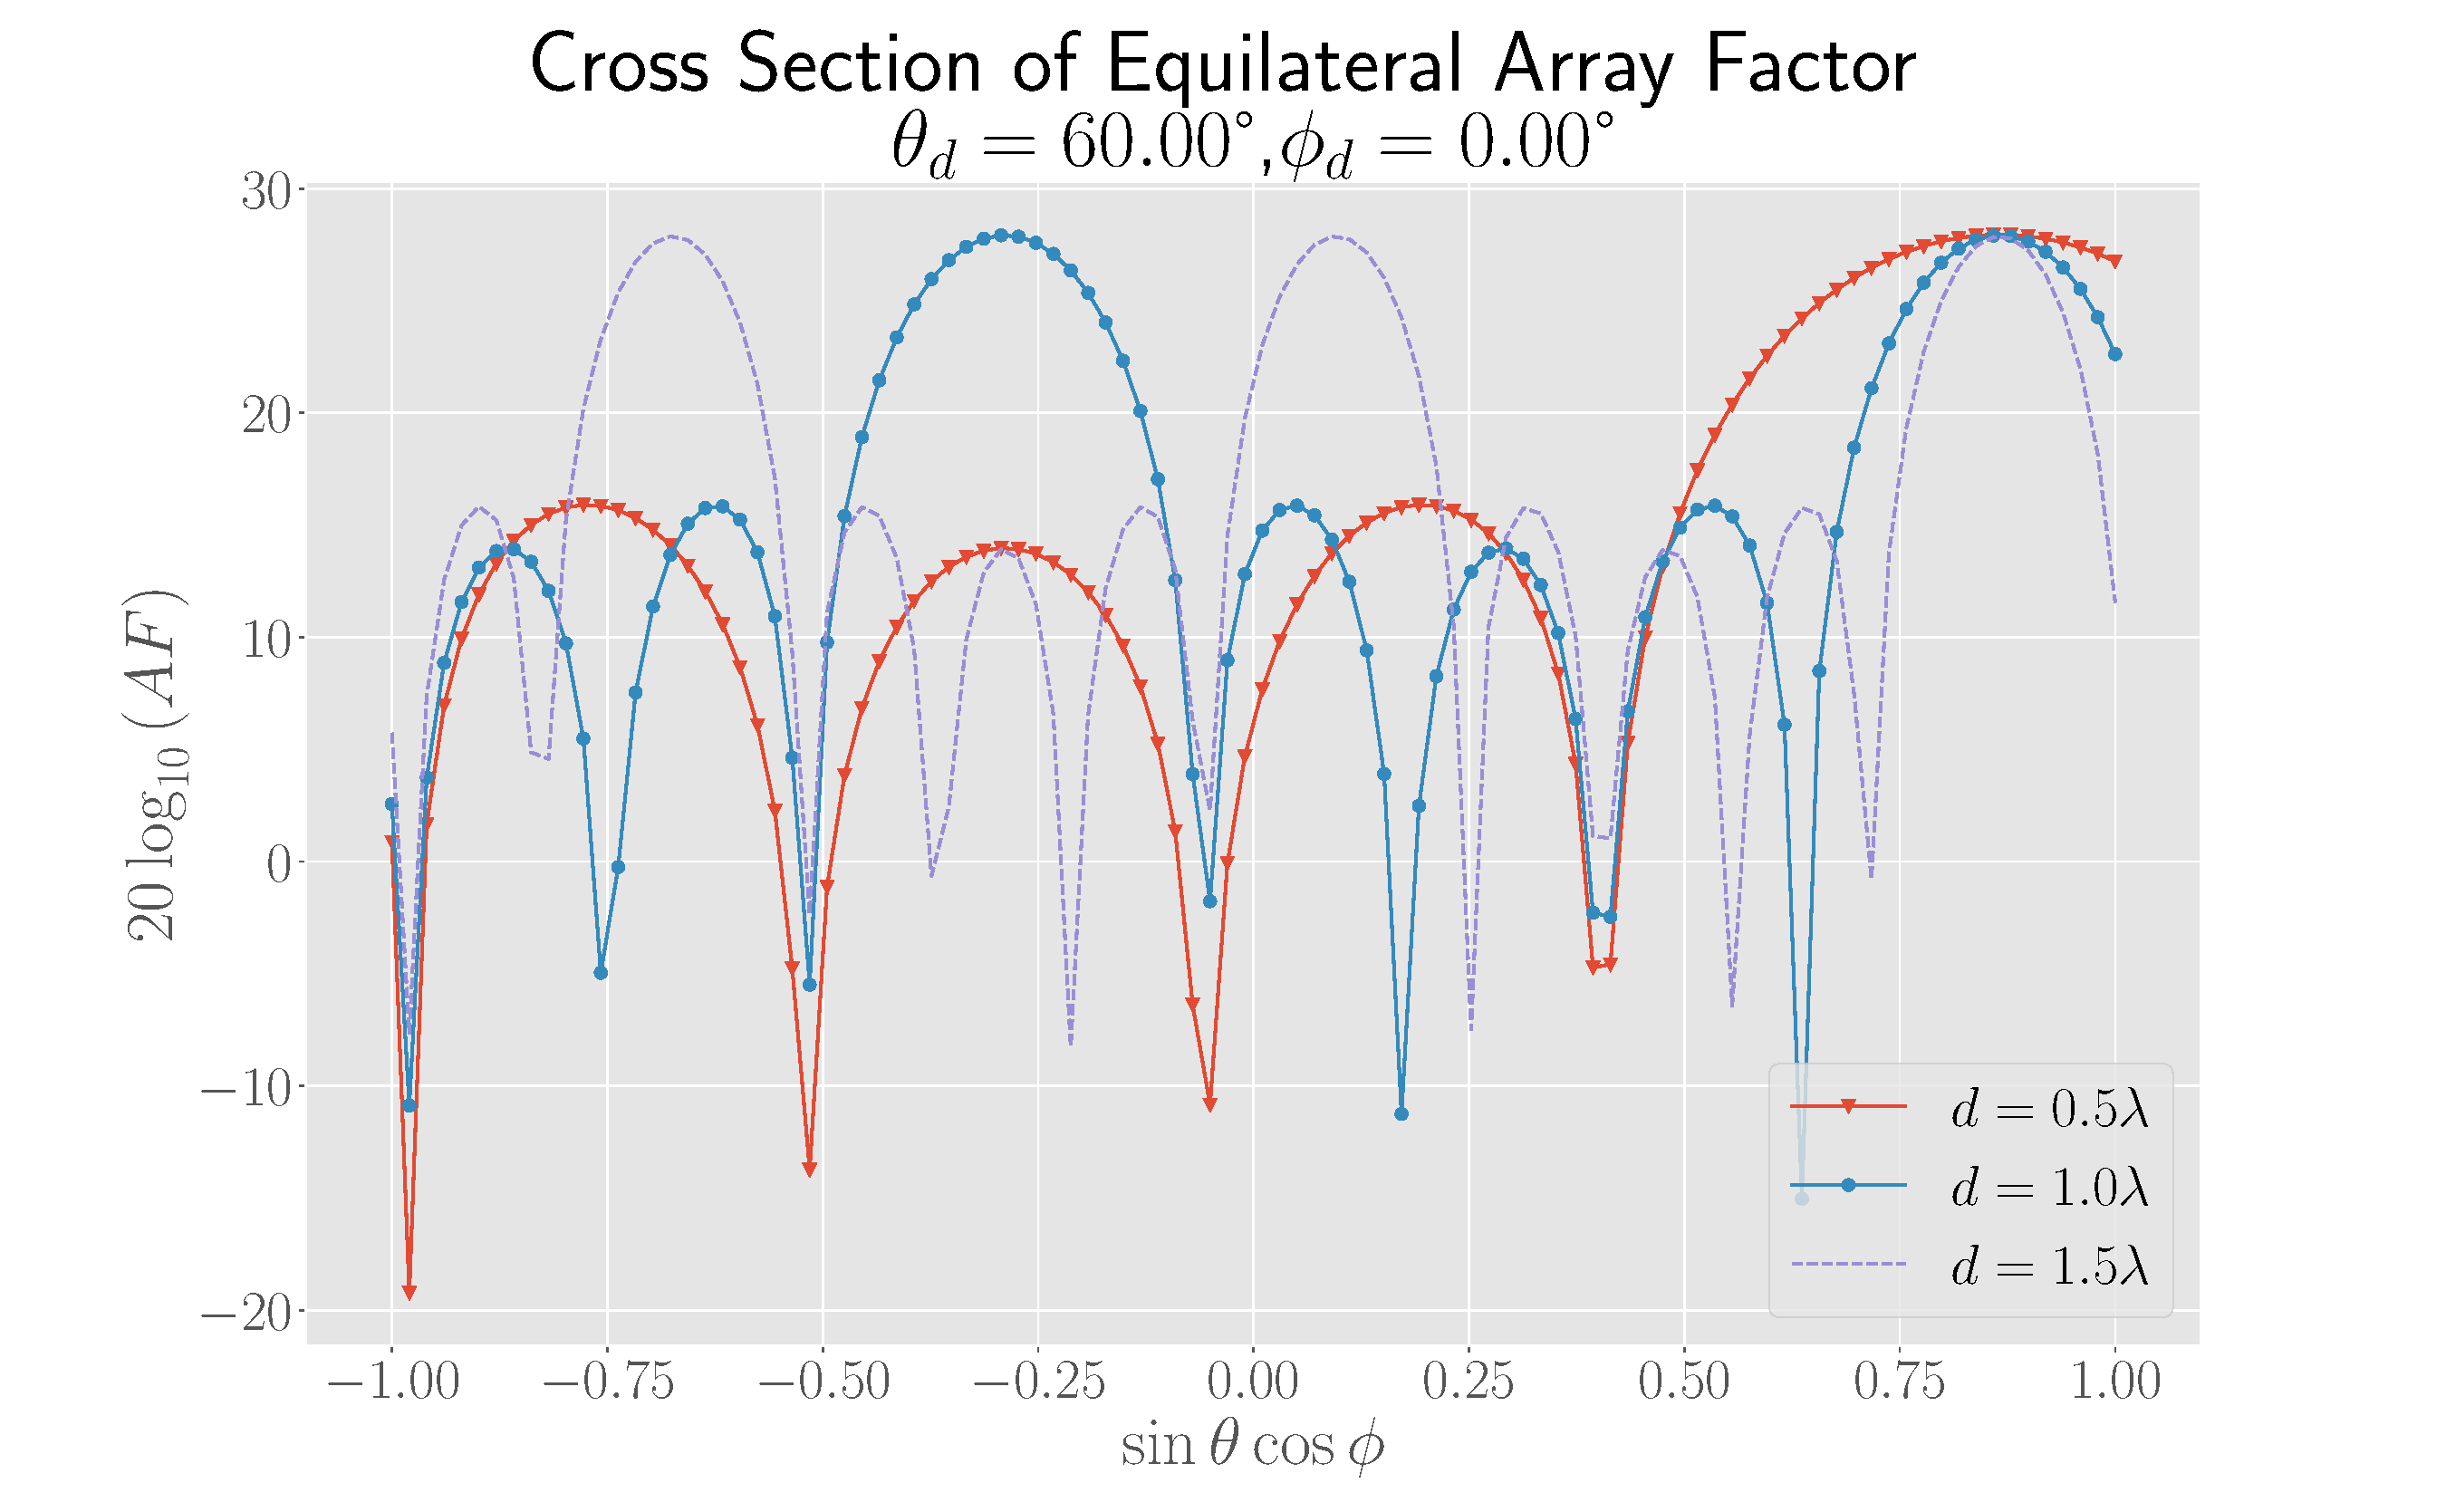
\includegraphics[width=0.618\textwidth]{graphics/task_3/equilat-60.00-theta-0.00-phi-cross.pdf}
    \caption{Comparison of cross-sections of the equilateral array factor for different spacings.}\label{fig:equilat-cross}
\end{figure}


\pagebreak

% ------------------------------------------------------------------------------

\printbibheading
\begin{refsection}[sources.bib]
\nocite{*}
\printbibliography[heading=subbibliography,title={Literature}]
\end{refsection}

\begin{refsection}[software.bib]
\nocite{*}
\printbibliography[heading=subbibliography,title={Software Used}]
\end{refsection}

\begin{refsection}[web.bib]
\nocite{*}
\printbibliography[heading=subbibliography,title={Web}]
\end{refsection}

\pagebreak
\appendix
\section{Python Code}\label{app:script}
\inputminted{python}{./code/square-array.py}

\end{document}
